% Copyright (c) 2008-2009 solvethis
% Copyright (c) 2010-2011 Casper Ti. Vector
% Public domain.

\documentclass[UTF8, oneside]{pkuthss}

% 使得打字机粗体可以被使用。
\usepackage{lmodern}
% 产生 originauth.tex 里的 \square。
\usepackage{amssymb}
% 提供 Verbatim 环境和 \VerbatimInput 命令。
\usepackage{fancyvrb}

% 解决无色彩时无法生成图片的问题
\usepackage{bmpsize}
% 控制图片位置
\usepackage{float}
% 插入代码
\usepackage{listings}
\lstset{
    tabsize = 4,
    frame = shadowbox, % lines OR shadowbox OR trBL
    numbers = left,
    numberstyle = \tiny,
    %basicstyle = \scriptsize,
    basicstyle = \footnotesize,
    breaklines = true,
    aboveskip = 1em
}

% 参考文献格式。
\bibliographystyle{ref/chinesebst-mod}
% 设定文档的基本信息。
\pkuthssinfo{
	cthesisname={硕士研究生学位论文},ethesisname={Undergraduate Thesis},
	ctitle={一种支持物理层WiFi安全\\研究的验证平台},
	etitle={A Verification platform for Physical Layer WiFi Security Research},
	cauthor={李晓光},
	eauthor={Xiaoguang Li},
	studentid={1401214261},
	date={二〇一七年五月},
	school={信息科学技术学院},
	cmajor={计算机系统结构},emajor={Computer Architecture},
	direction={无线局域网体系结构},
	cmentor={王韬},ementor={Prof.\ Tao Wang},
	ckeywords={WiFi安全,物理层,无线验证平台},
	ekeywords={WiFi security, physical layer, verification platform},
}

% 清理tex local的命令:mktexlsr

\begin{document}
	% 以下为正文之前的部分。
	\frontmatter

	% 自动生成标题页。
	\maketitle

	% 版权声明。
	% Copyright (c) 2008-2009 solvethis
% Copyright (c) 2010-2011 Casper Ti. Vector
% All rights reserved.
%
% Redistribution and use in source and binary forms, with or without
% modification, are permitted provided that the following conditions are
% met:
%
% * Redistributions of source code must retain the above copyright notice,
%   this list of conditions and the following disclaimer.
% * Redistributions in binary form must reproduce the above copyright
%   notice, this list of conditions and the following disclaimer in the
%   documentation and/or other materials provided with the distribution.
% * Neither the name of Peking University nor the names of its contributors
%   may be used to endorse or promote products derived from this software
%   without specific prior written permission.
%
% THIS SOFTWARE IS PROVIDED BY THE COPYRIGHT HOLDERS AND CONTRIBUTORS "AS
% IS" AND ANY EXPRESS OR IMPLIED WARRANTIES, INCLUDING, BUT NOT LIMITED TO,
% THE IMPLIED WARRANTIES OF MERCHANTABILITY AND FITNESS FOR A PARTICULAR
% PURPOSE ARE DISCLAIMED. IN NO EVENT SHALL THE COPYRIGHT HOLDER OR
% CONTRIBUTORS BE LIABLE FOR ANY DIRECT, INDIRECT, INCIDENTAL, SPECIAL,
% EXEMPLARY, OR CONSEQUENTIAL DAMAGES (INCLUDING, BUT NOT LIMITED TO,
% PROCUREMENT OF SUBSTITUTE GOODS OR SERVICES; LOSS OF USE, DATA, OR
% PROFITS; OR BUSINESS INTERRUPTION) HOWEVER CAUSED AND ON ANY THEORY OF
% LIABILITY, WHETHER IN CONTRACT, STRICT LIABILITY, OR TORT (INCLUDING
% NEGLIGENCE OR OTHERWISE) ARISING IN ANY WAY OUT OF THE USE OF THIS
% SOFTWARE, EVEN IF ADVISED OF THE POSSIBILITY OF SUCH DAMAGE.

\chapter*{版权声明}
{

	任何收存和保管本论文各种版本的单位和个人,
	未经本论文作者同意,不得将本论文转借他人,
	亦不得随意复制、抄录、拍照或以任何方式传播。
	否则一旦引起有碍作者著作权之问题,将可能承担法律责任。

}

	% 中英文摘要。
	% Copyright (c) 2008-2009 solvethis
% Copyright (c) 2010-2011 Casper Ti. Vector
% Public domain.

\begin{cabstract}

	现代社会中,WiFi作为一种快速、便捷、不考虑流量的无线上网方式,成为人们基本的生活需求,WiFi接入点遍布家庭、企业、公共场所等区域。
	WiFi的普及也为人们的网络生活带来了安全隐患,一些不法分子通过WiFi向用户发起攻击。
	现有的WiFi加密协议包括WEP、WPA和WPA2等存在安全漏洞,有被破解的可能,
	有的攻击者破解个人WiFi的密码,目的是占用网络资源,降低合法用户的服务质量,俗称“蹭网”。
	另有一些攻击者利用带无线网卡的电脑和网络分析软件搭建钓鱼WiFi,监听网络报文,
	获取用户手机号、网站账号、密码等敏感信息,甚至可以窃取钱财,给用户带来巨大损失。

	为了检测和阻止层出不穷的攻击,针对WiFi安全的研究广泛开展。
	近年来,结合物理层的安全机制成为WiFi安全研究的热点,物理层含有丰富的无线信道、设备位置、信号质量等信息,
	研究者探索如何利用这些信息加强WiFi的安全性。

	WiFi安全的研究需要有开发和验证平台,用以实现和评估研究成果。
	物理层的安全研究对验证平台提出很高的要求,由软件实现的WiFi物理层无法满足协议对性能的要求,而硬件实现的物理层往往不可编程。
	从近些年的研究看,验证平台的质量常常成为制约研究成果有效性的瓶颈,
	一些验证平台不支持物理层的编程,一些验证平台延迟过高无法与商用WiFi设备实时通信。
	“工欲善其事,必先利其器”,支持物理层编程的高性能WiFi验证平台成为WiFi安全研究必不可少的工具。

	本文对近年来物理层WiFi安全的研究进行了深入分析,总结了这些研究对验证平台的需求,
	设计了一种支持物理层WiFi安全研究的验证平台GRTSEC,并利用商用设备进行了实现,
	结合实际的使用样例论证了可以满足物理层WiFi安全研究的需求。
	% 作为使用样例,基于此平台搭建了伪装WiFi,并验证了利用物理层信息对WiFi设备进行识别技术的可行性。

\end{cabstract}

\begin{eabstract}
	In modern society, WiFi is people's basic needs of life.
	As a fast, convenient, cheap wireless access to Internet, WiFi access point spread all over the home, business, public places.
	WiFi popularity for people's network life has brought security risks, some people attack the user through WiFi.
	Existing WiFi encryption protocols include WEP, WPA and WPA2 have security vulnerabilities, there is the possibility of being cracked.
	Some attackers crack personal WiFi password, the purpose is to take up network resources,
	reduce the quality of legitimate users of the service, commonly known as "rub network."
	Some other attackers use the commercial computer and network analysis software to build phishing WiFi,
	monitor network packets, access to mobile phone number, website account, password and other sensitive information,
	and even steal money, which bring to the user a huge loss.

	In order to detect and prevent the endless attacks, WiFi security researches are carried out extensively.
	In recent years, the security mechanism combined with the physical layer has become the new interest of WiFi security research.
	The physical layer contains rich information such as wireless channel information, device location and signal quality.
	Researchers explore how to use these information to enhance WiFi security.

	WiFi security researches require a development and verification platform to implement and evaluate research results.
	The physical layer of security research on the verification platform made a high demand,
	by the software to achieve the WiFi physical layer can not meet the requirements of the real-time communication,
	while hardware implementation is often poor programmability.
	In recent years, the quality of the verification platform has often become a bottleneck in restricting the effectiveness of research results.
	Some verification platforms do not support the programming of the physical layer.
	Some of the verification platforms are too slow to communicate with commercial WiFi devices in real time.
	To support the physical layer programming high-performance WiFi verification platform for WiFi security research is an indispensable tool.

	In this paper, we study the research on WiFi security of physical layer in recent years,
	and summarize the requirements of verification platform.
	A verification platform called GRTSEC supporting the study of WiFi layer security is designed and implemented by commercial device.
	This paper demonstrates the need to meet the needs of most physical layer WiFi security research,
	and builds a camouflage WiFi based on this platform, and proposed a WiFi device identification technology with physical layer information .

\end{eabstract}

	% 自动生成目录。
	\tableofcontents

	% 以下为正文。
	\mainmatter

	% 各章节。
	% Copyright (c) 2008-2009 solvethis
% Copyright (c) 2010-2011 Casper Ti. Vector
% Public domain.

\chapter{引言}
	\section{课题背景与研究意义}

		现代社会中,WiFi作为一种快速、便捷、不考虑流量的无线上网方式,成为人们基本的生活需求,WiFi接入点遍布家庭、企业、公共场所等区域。
		WiFi的普及为人们的网络生活带来了安全隐患,一些不法分子通过WiFi向用户发起攻击。
		相对于有线网络,无线网络的通信内容广播到空气中,安全性较低。
		现有的WiFi加密协议包括WEP、WPA和WPA2等存在安全漏洞,存在被破解的可能\cite{wisec09wep}。
		有的攻击者破解个人WiFi的密码,目的是占用网络资源,降低合法用户的服务质量,俗称“蹭网”。
		另有一些攻击者利用带无线网卡的电脑和网络分析软件搭建钓鱼WiFi,监听网络报文,
		获取用户手机号、网站账号、密码等敏感信息,甚至可以窃取钱财,给用户带来巨大损失。
		在2015年的央视3·15晚会上,网络安全工程师伪装了演播室的免费WiFi,钓鱼得到的现场观众的信息,
		观众自拍的照片和邮箱密码竟出现在了演播室大屏幕上\cite{cctv315}。
		普通用户有时为了占用更多的无线网络带宽,也会有意或无意地向同网其它用户发起攻击,损害其它用户的网络质量\cite{tifs12reciprocity}。

		为了检测和阻止层出不穷的攻击,针对WiFi安全的研究广泛开展。
		近年来,结合物理层的安全机制成为WiFi安全研究的热点,物理层含有丰富的无线信道、设备位置、信号质量等信息,
		研究者探索如何利用这些信息加强WiFi的安全性,
		例如基于RSS(Received Signal Strength,接收信号强度)和CSI(Channel State Informatica,信道状态信息)的密钥生成策略\cite{access16key},
		基于RSS的物理层认证策略\cite{ieeewc10noncryp},
		基于CIR(Channel Impulse Response,信道冲激响应)的物理层认证技术\cite{milcom11cir, icc13cir},
		基于信道频率响应特性的物理层指纹和窃听检测技术\cite{icc07xiao, globecom10xiao}等。

		WiFi安全的研究需要有开发和验证平台,用以实现和评估研究成果。
		相对于上层的安全研究,物理层的安全研究对验证平台提出很高的要求,
		802.11a/g协议中规定的物理层数据传输速率为54Mbps,延迟为16$\mu s$,软件实现的物理层无法在速率和延迟上满足要求,
		而硬件实现往往可编程性较差,开发和调试周期长,缺少可供参考的工具库。
		从近些年的研究看,验证平台的质量常常成为制约研究成果有效性的瓶颈,
		一些验证平台不支持物理层的编程,一些验证平台延迟过高无法与商用WiFi设备实时通信\cite{mobicom13securearray}。
		“工欲善其事,必先利其器”,支持物理层编程的高性能WiFi验证平台成为WiFi安全研究必不可少的工具。

		现有支持物理层WiFi研究的无线开放平台按物理层实现方式和编程方式主要分为四类:
		\begin{itemize}
			\item 计算机仿真软件,没有射频前端,物理层由纯软件实现,支持软件编程,有较多的参考样例,代表是Matlab;
			\item 商用网卡,有射频前端,物理层由ASIC实现,不支持软件编程但支持软件配置,代表是Intel 5300;
			\item 软件无线电平台,有射频前端,物理层由软件实现,支持软件编程,有较多的参考样例,代表是NI公司的硬件USRP与软件GNU Radio或LabVIEW的组合;
			\item 基于FPGA的无线电开放平台,有射频前端,物理层由FPGA实现,部分支持软件编程,参考样例少,代表是莱斯大学的WARP平台;
		\end{itemize}

		各类平台在可编程性和性能上各有优势,但目前没有平台在性能和可编程性上同时很好地满足近年来物理层WiFi安全研究,
		具体体现在没有平台在满足802.11协议规定的速率和延迟的同时,可以提供给研究者物理层的高可编程性。
		因此,物理层WiFi安全的研究者需要一个无线开放平台,在性能和可编程性上同时满足研究需求,用以实现和验证研究内容。

	\section{主要研究内容}
		本文的基本目标是为物理层WiFi安全的研究者提供一个无线验证平台GRTSEC(GRT for Security),
		围绕基本目标,本文的主要研究内容有以下几点:
		\begin{itemize}
			\item 对WiFi安全进行调研,总结常见的WiFi攻击以及WiFi安全相关的最新研究成果,分析WiFi安全研究对验证平台的需求;
			\item 对常见的WiFi验证平台进行调研,对各类平台进行对比和分析,找到各平台的优势以及不足;
			\item 设计适用于WiFi安全研究的框架,并基于FPGA进行实现;
			\item 为本文提出的验证平台设计使用样例,根据使用样例论证验证平台可以满足WiFi安全研究的需求;
			\item 使用本文提出的验证平台,搭建伪装WiFi,并提出一种新型的物理层WiFi识别技术识别不同WiFi设备。
		\end{itemize}

	\section{本文贡献}
		本文主要有以下贡献:
		\begin{itemize}
			\item 对物理层WiFi安全相关研究进行调研,分析了对WiFi验证平台的需求及现有系统的不足,
			定义了作为WiFi安全研究验证平台所需具有的特性;
			\item 在现有系统的基础上,设计并实现了一种支持物理层WiFi安全研究的验证平台,
			性能上满足与商用设备通信的要求,提供易于编程调用的API;
			% 通过使用样例论证了本文提出的验证平台可以满足绝大多数物理层WiFi安全研究的需求;
			\item 作为使用样例,提出了一种新型的物理层WiFi识别技术,可以对不同WiFi设备进行识别,
			利用本文提出的验证平台,在与商用设备实时通信中验证了其有效性。
		\end{itemize}

	\section{本文组织}
	第二章对WiFi安全相关的背景进行介绍;
	第三章对WiFi安全研究进行需求分析,提出了设计目标;
	第四章是验证平台的具体设计与其FPGA实现;
	第五章是验证平台使用样例的介绍,包括对已有研究的支持和新的安全认证技术;
	第六章是性能测试与评估,对平台的性能进行详细测试,对结果进行分析;
	第七章是文章总结与下一步研究的展望。

	% Copyright (c) 2008-2009 solvethis
% Copyright (c) 2010-2011 Casper Ti. Vector
% Public domain.

\chapter{背景介绍与相关工作}
本章将介绍WiFi的背景、WiFi安全的研究进展以及相关的WiFi验证平台。
本章首先在\ref{sec:comm_principle}节、\ref{sec:80211protocol}节介绍WiFi的背景知识,
然后在\ref{sec:security_research}节介绍物理层WiFi安全相关的研究,
其次在\ref{sec:related_work}节介绍现有的WiFi验证平台,
最后在\ref{sec:chap2_conclusion}节对本章进行小结。

	\section{WiFi物理层信息}\label{sec:comm_principle}
	研究者利用物理层信息加强WiFi的安全性,不同的物理层信息各有特点。
	本节介绍在WiFi安全研究中常见的几种物理层信息及其在无线通信中的物理意义。
		\subsection{RSS与RSSI}
		RSS(Received Signal Strength)是接收信号强度,指WiFi接收机收到的信号的功率,
		单位为dBm,为负数,越接近0表示信号质量越高。
		RSSI(Received Signal Strength Indicator)是接收信号强度指示,是无单位的。
		RSS一般为负值不太直观,人们把RSS人为映射为正值RSSI,理解和比较起来更直观,
		一般WiFi系统呈现给用户的是RSSI,不同系统有不同的映射方式\cite{wikirssi}。
		RSSI本质上与RSS只是同一个物理层信息的不同表示方法,文献里用二者都会出现,本文以RSSI进行表示。

		RSSI与无线发射机功率、收发距离、周围障碍物环境有关,发射机功率越大、收发距离越短,RSSI越大,而RSSI与障碍物环境关系比较复杂。
		不同的位置来源的信号一般RSSI也不同,因此无线通信的研究者常常通过RSSI获取相对位置。

		\subsection{CSI与CIR}\label{sec:background_csi}
		CSI(Channel State Information)是信道状态信息,是无线通信中从发射机到接收机之间信道的属性。
		在无线通信中,接收机接收到的信号与发送信号不完全相同,存在环境引起的变化,
		环境的影响称为信道,接收信号是发送信号与信道共同作用的结果,如式\ref{math:channel_model},
		\begin{equation}
			\centering
			r(t)=h(t)*s(t)+n
			\label{math:channel_model}
		\end{equation}
		$r(t)$代表接收信号,$h(t)$代表信道,$s(t)$代表发送信号,$n$代表噪声。

		接收机为了从接收信号中还原出发送信号,需要先得到信道信息,然后消除信道对接收信号的影响。
		接收机得到的信道信息,称作CSI。
		为了得到CSI,无线通信中常采用的方法是发射机发送一段双方已知的信号,称为训练序列,接收机对比接收信号和理论信号,
		得到信道信息,这个过程称为信道估计,从接收信号中消除信道影响的过程称为补偿\cite{book06commprin}。
		这里基于的一个假设是在短时间内信道变化不大,信道对训练序列的作用与信道对信号其它部分的作用相近。

		影响CSI的因素很多,有多径效应、多普勒效应、随距离的能量衰减等。
		多径效应是指由于周围物体的反射,信号经过多条路径到达接收机,每条路径效果叠加称为多径效应\cite{book06commprin}。
		多普勒效应是由发射机和接收机之间相对位置的变化引起。
		CSI具有丰富的物理内涵,常常被无线研究者用来推测其它信息,比如判断位置、判断是否有人经过、判断是否在移动。

		有的文献中也具体标明使用CIR这个物理量,CIR(Channel Impulse Response)是信道冲激响应,是一种特殊的CSI
		表示发送端发送一个脉冲信号的时候,接收端所能收到的信号值$h(t)$。
		CIR通常表示时域的信道特征,CSI既包含时域特征,也包含频域特征,是信道信息的总称。

		\subsection{频率偏移}
		介绍频率偏移之前,首先介绍频率同步。同步是指无线通信系统的接收机从收到的波形中找出有效信号,是无线通信中必不可少的步骤。
		同步分为两类,时间同步和频率同步。时间同步是指找到发送信号的起始时间,对于异步的通信系统都需要进行时间同步,如串口通信协议。
		接收信号和发送信号的载波频率存在频率偏移(简称频偏),频率同步是指找到并补偿频率偏移,还原出发送信号。
		频偏对频分复用系统会造成很严重的影响,因此频率同步是频分复用系统必要的组成部分。

		\begin{figure}[H]
			\centering
			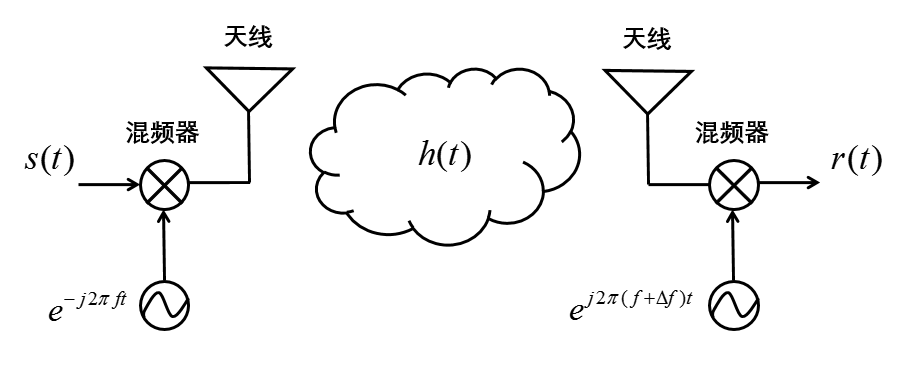
\includegraphics[width=0.7\textwidth]{img/freq_offseet_channel_model.png}
			\caption{无线通信系统中频率偏移的信道模型}
			\label{fig:freq_offseet_channel_model}
		\end{figure}
		频偏的信道模型可以由图\ref{fig:freq_offseet_channel_model}表示,$s(t)$表示发送的基带信号,$r(t)$表示接收的基带信号,$h(t)$表示信道,
		混频器用来将基带信号与载波合成后搬移到射频上,图中省略了低噪声放大器等其他通信电路。
		如图\ref{fig:freq_offseet_channel_model}所示,频率偏移由接收机和发射机载波频率不一致引起,
		设发射机载波频率为$f$,接收机载波频率为$f+\Delta f$,$\Delta f$为频率偏移。
		频偏的数学模型可以表示为式\ref{math:freq_offset},噪声对频偏几乎没有影响,
		\begin{equation}
			\centering
			r(t)=h(t)*s(t) \cdot e^{-j2\pi ft} \cdot e^{j2\pi(f+\Delta f)t}
			\label{math:freq_offset}
		\end{equation}
		对于实际的无线通信系统,常常使用有周期性的训练序列进行频偏估计,根据周期的偏移推测频率偏移,然后进行频偏补偿。

	\section{802.11协议简介}\label{sec:80211protocol}
	WiFi通信的协议是IEEE 802.11协议集,规定了MAC(媒体访问控制)层和物理层的规范,
	具体协议按推出的时间顺序有802.11b、802.11a、802.11g、802.11n、802.11ac等。
	目前市面上的主流WiFi芯片都支持802.11a/g/n协议,本文主要基于802.11a/g/n协议进行阐述。
		\subsection{802.11物理层介绍}
		802.11物理层规定了数据传输的调制解调方式、编码方式、射频参数等,是OSI网络模型的最底层。
		除802.11b使用DSSS(direct-sequence spread spectrum,直接序列扩频)调制技术外,
		802.11a/g/n/ac等都使用了OFDM(Orthogonal frequency-division multiplexing,正交频分复用)调制技术。

		OFDM是一种将信号分配到多个子载波的频分调制方式,每一个子载波的调制后信号有部分重叠,但因为子载波之间严格正交,接收机可以分离出不同子载波的信号。
		OFDM的优点是在子载波间不需要保护间隔,频谱利用率高,且抗多径衰落能力强,
		缺点是对频率偏移敏感,需要对频偏进行纠正\cite{book06commprin}。
		OFDM由于其对复杂环境的抗干扰性,目前广泛应用于宽带通信,如WiFi、4G移动网络、数字电视、非对称数字用户环路(ADSL)等。
		802.11a/g协议规定的OFDM子载波数量为64个,其中传输数据的子载波是48个,传输导频的子载波是4个,
		802.11n协议20M带宽模式下子载波数量为64个,其中传输数据的子载波是52个,传输导频的子载波是4个,
		802.11n协议高吞吐率40M带宽模式下子载波数量为128个,其中传输数据的子载波是108个,传输导频的子载波是6个\cite{ieee80211}。

		\begin{figure}[H]
			\centering
			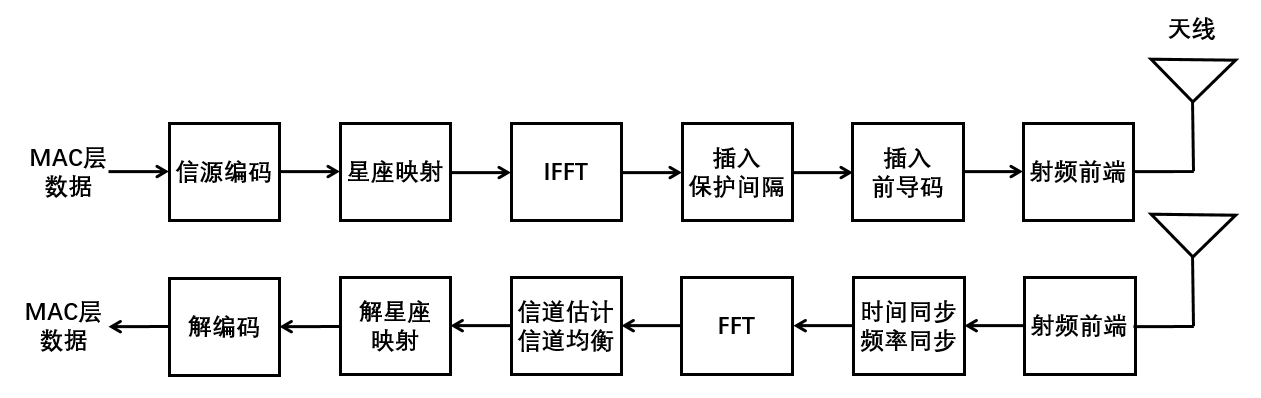
\includegraphics[width=0.7\textwidth]{img/80211_phy_module.png}
			\caption{802.11a/g物理层的简单模块示意图}
			\label{fig:80211_phy_module}
		\end{figure}
		图\ref{fig:80211_phy_module}是802.11a/g物理层的简单模块示意图,802.11n在此基础上增加对多天线的支持。
		发送端得到来自MAC层的数据,经过信源编码、星座映射、IFFT(Inverse Fast Fourier Transform,快速傅里叶逆变换)、插入保护间隔、插入前导码、射频前端到达空气中。
		其中,信源编码包括扰码、冗余编码、交织等步骤,目的是使信源数据更加强健;
		星座映射是将二进制数据映射到复数星座点上,有不同的映射策略,对应多种调制方式;
		IFFT是OFDM的关键步骤,将频域信号转变为时域信号,对于802.11a/g,此处是64点IFFT,对于802.11n,此处兼有64点IFFT和128点IFFT;
		插入保护间隔是指在时域的不同符号间插入一段间隔时间,降低码间串扰的影响;
		插入前导码是指在一帧前面增加训练字,如\ref{sec:comm_principle}节所述,训练字用来完成时间同步、频率同步、信道估计等功能。
		接收端从空气中得到无线信号,经过射频前端得到复数表示的I/Q两路信号,经过时间同步和频率同步后得到一帧,
		去掉保护间隔后经过FFT得到频域信号,经过信道估计和信道均衡后去除信道对信号的影响,
		经过解星座映射后由复数信号得到二进制数据,经过解码还原出真实数据,传给MAC层。

		802.11物理层中蕴含了很多对于WiFi安全研究有价值的信息,尤其是接收端模块,比如信道估计模块可以得到CSI,反映了发射机的位置、周边环境等,
		频率同步模块可以得到频率偏移,解星座映射模块可以得到接收信号的星座图。

		\subsection{802.11 MAC层介绍}
		在OSI网络模型中,物理层之上的一层是数据链路层,MAC层是数据链路层的子层,802.11协议规定的是物理层和MAC层的规范。
		MAC层提供了在不可靠的无线媒介中可靠传输用户数据的机制。本文主要面向物理层,会简单涉及MAC层,此处只对MAC层做简单介绍。

		802.11 MAC层有两种功能规范,必须具备的功能DCF(Distributed Coordination Function,分布式协调功能)
		和可选功能PCF(Point Coordination Function,集中式协调功能)。
		DCF主要基于CSMA/CA(Carrier sense multiple access with collision avoidance,带碰撞避免的载波侦听多址)技术。
		CSMA/CA技术是指一个无线节点在发送数据之前,首先侦听当前载波上是否有其他设备使用,只有没有其他人发送时可以发送数据。
		当有其他人发送数据时,首先等到空闲,然后再等待随机一段时间空闲后再发送,随机等待机制称为随机回退\cite{citsa05backoff}。

		\subsection{802.11安全机制}\label{subsec:80211security}
		802.11协议在MAC层规定了安全机制。
		1997年推出的最初的802.11协议将WEP(Wired Equivalent Privacy)认证方式应用于MAC层规范,
		后来在2003年,WiFi联盟提出WPA(Wi-Fi Protected Access)认证方式,
		在2004年,随着IEEE推出802.11i协议规定了WPA2认证方式,WEP认证被弃用\cite{wikiwep},
		在2012版802.11协议中,只保留WPA2认证方式,即802.11i协议\cite{ieee80211}。

		WEP和WPA被802.11协议弃用是因为其强度低易被破解,然而,WPA2认证方式也存在被攻击的可能。
		\cite{ijarcet12wpa2}中研究了WEP、WPA、WPA2的漏洞,并利用软件Aircrack-ng演示了如何破解这三种认证方式。
		MAC层安全机制的不完备性驱动越来越多的研究者开始探索物理层的安全机制,在第\ref{sec:security_research}节会介绍相关研究。

	\section{物理层WiFi安全研究进展}\label{sec:security_research}
	本节首先在\ref{subsec:attack_model}小节介绍WiFi攻击模型的研究进展,提出新的攻击模型是巩固WiFi安全的一种方式;
	其次介绍物理层WiFi安全机制的研究进展,研究者利用物理层信息进行用户的认证和设备的识别,
	物理层安全机制分为基于加密技术的安全机制和非加密安全机制,基于加密技术的安全机制在\ref{subsec:phy_tech_key_generation}小节进行介绍,
	非加密安全机制可以宽泛地分为硬件指纹技术和信道指纹技术\cite{ieeewc10noncryp}\cite{mobicom08radiometric},分别在
	\ref{subsec:phy_tech_device_fingerprint}、\ref{subsec:phy_tech_channel_fingerprint}小节进行介绍。
		\subsection{WiFi攻击模型的研究进展}\label{subsec:attack_model}
		相对于有线网络,无线网络的开放性给攻击者带来了可乘之机。针对WiFi的攻击按主动性可分为被动攻击和主动攻击。
		被动攻击主要是窃听获取密码,
		例如,通过监听CSI和上层网络报文,可以推测出用户在手机支付时输入的密码\cite{ccs16csi};
		通过窃听相邻设备的信道信息,获取基于信道的加密密钥\cite{ccs07robustkey}。
		主动攻击有欺骗攻击、DoS(Denial of Service,拒绝服务)攻击、密钥破解等,
		例如:攻击者伪装成合法设备MAC地址,只用10秒钟向AP发送去认证包,可使合法设备数分钟内无法连接AP\cite{usenix03dos};
		攻击者产生大量随机MAC地址向AP发送连接请求,消耗网络资源,可使DHCP服务器可分配IP被全部消耗\cite{wisec06spoofing};
		攻击者发起DoS攻击,不停地发送干扰信号,使合法设备之间无法正常通信\cite{milcom13jamming, jsac12antijamming};
		信号注入攻击可以破解密钥,攻击者通过向密钥达成一致的两台设备之间注入无线信号,
		使合法设备生成被自己控制的密钥,攻击者很大概率可以猜出密钥\cite{cns15key}。

		\subsection{物理层密钥技术}\label{subsec:phy_tech_key_generation}
		物理层密钥技术是指利用物理层信息生成密钥,对通信内容进行加密。
		对于密钥加密的无线通信系统,如何共享密钥是一个挑战,因为无线环境是开放的、公共的,攻击者可以轻易地监听到交换密钥的过程。
		无线通信中的密钥生成需要满足三个原则,时变性、互惠性、空间不相关性\cite{access16key}。
		时变性是指短时间内不变,一段时间后会发生变化,使密钥具有时效性;互惠性是指加密通信双方可以得到同一个密钥;空间不相关性指不同空间的设备得到不同的密钥。
		物理层的信道信息(RSSI或CSI)满足这三个原则,WiFi的通信双方之间共享同一个无线信道,会随时间变化,不同位置的信道不同,
		因此信道信息常常被用于密钥生成。

		例如,有文章讨论了基于RSS和CSI的密钥生成策略\cite{access16key},这篇文章研究了信道条件和信道参数对密钥生成的影响,分析得出RSS和CSI均可用于密钥生成,
		但基于RSS的密钥系统易受预测攻击,而基于CSI的不受此攻击影响。
		另有研究讨论了在信道互惠性无法满足时如何用CSI生成密钥\cite{infocom13key},
		提出使用信道增益补偿(Channel Gain Complement)的方法达成密钥一致。
		有文章提出向信道引入随机信号的密钥生成方法\cite{cns15key},合法设备A向合法设备B发送训练序列时,加入本地生成的一个均值为0的随机信号$X$,
		B收到时将信道值$H$乘以自己的随机信号$Y$,这样双方可以得到共同的密钥$XYH$,攻击者无法同时得到双方的随机信号。

		\subsection{硬件指纹技术}\label{subsec:phy_tech_device_fingerprint}
		硬件指纹技术是指利用硬件相关的物理层信息进行识别和认证的技术,这里的硬件主要指WiFi发射机和接收机的电路。
		在无线通信中,数据容易伪造,电路的固有属性难以模仿和复制,因此,硬件相关的物理层信息常常用来进行身份的识别。
		WiFi中硬件相关的物理层信息有时钟偏移、时钟波动、射频特性等。

		PARADIS系统\cite{mobicom08radiometric}利用多种物理层信息结合机器学习对802.11无线设备进行识别。
		硬件电路上的不完美性会引起射频信号的偏移,这篇文章收集与设备硬件关系紧密的物理层信息,
		包括频偏、训练字段与理论值的相关性、星座图中星座点的偏移,接收端提取这些特征与设备对应,作为训练集,由机器学习的方法对新收到的包进行判断。
		为了提高准确度,对多个连续的包取平均,这里与信道指纹技术结合,保证多个连续的包具有相同的信道指纹。
		这篇文章的实验表明,PARADIS系统可以识别超过130种商用网卡,准确度超过99\%。

		也有其他无线系统,如蓝牙,采用硬件指纹技术进行身份识别。
		例如BlueID系统\cite{infocom14blueid}利用蓝牙设备的时钟不同特性进行设备识别。

		\subsection{信道指纹技术}\label{subsec:phy_tech_channel_fingerprint}
		信道指纹技术是指利用信道相关的物理层信息进行识别和认证的技术,这里的信道指无线通信的信道,参见\ref{sec:background_csi}。
		在无线通信中,信道与调制方式、射频参数、周围环境等关系密切,
		因此,信道相关的物理层信息常常用来定位和判断设备是否被移动,在短时间内,也可以用来进行身份识别。
		信道相关的物理层信息有CSI、RSSI、多天线信号方向矩阵等。

		有研究利用RSSI对无线设备进行认证\cite{wisec06spoofing},具体来说,多个AP连接到一个称作WA(wireless appliance)的中心服务器上,
		AP将每一个成功接收的包的RSSI汇总给WA,由WA进行记录和认证,多个AP对同一个包记录的RSSI组成向量$S$,称作信号指纹(signalprint),
		$S_i$表示第$i$个AP记录的RSSI,若第$i$个AP没有收到此包,记录为默认最小值-95$dBm$。
		如果AP数量不足以在同一信道布置多台,则当发现有可疑包时(如去认证包)再将其他信道的AP调整到信道。
		此方法还可以用来识别同一台设备产生大量随机MAC引起的DoS攻击,因为同一台设备发出的包会拥有相近的信号指纹。
		这篇文章的方法有较大局限,比如多数实际场景不具备多台AP,待检测的设备不能移动,无法检测距离合法用户5米范围内的攻击者等。

		有研究提出利用CSI检测物联网设备是否是非法移动\cite{acsac15iot}。
		一些场景下物联网设备不希望被其他人移动,比如植物监控摄像头、办公室摄像头等。
		这篇文章利用CSI是否变化来判断设备是否被移动,需要与人员走动进行区别,
		具体方法是用多接收端区分环境变化和设备移动,如果是设备移动,会对所有接收端造成影响,如果是环境变化,不会对所有接收端影响。

		有研究提出利用多天线的CSI识别多种主动攻击\cite{mobicom13securearray}。
		多天线技术在802.11n协议开始使用,可以显著地提高系统传输速率和准确度。
		这篇文章利用多天线的CSI提取出信号到达角度,提出一套通过到达角度认证的DataCheck协议,对设备进行识别和认证。
		可以识别相隔5厘米的设备,相对于利用RSSI的识别距离5米\cite{wisec06spoofing},识别精度明显提高,
		而且多天线技术可以替代布置多设备,降低成本。

		\subsection{本节小结}
		本节首先介绍了常见的WiFi攻击,然后介绍了三种利用物理层信息应对WiFi攻击的策略,密钥技术、硬件指纹技术、信道指纹技术。
		其中密钥技术主要对802.11现有加密机制进行改进,提高传输内容的安全性,适合在商用802.11网卡上进行部署。
		硬件指纹技术和信道指纹技术都可以对设备进行身份验证,都是先学习再识别的模式,
		其中硬件指纹技术对学习过程的要求比较高,常常需要机器学习的技术,但可以应对设备移动的场景,
		信道指纹技术主要在短时间内对静止的设备进行识别。

	\section{现有的WiFi验证平台}\label{sec:related_work}
	在物理层WiFi安全的研究中,常见的验证平台主要分为四类:计算机仿真软件,商用网卡,软件无线电平台,基于FPGA的无线电开放平台。
	不同平台各有优劣,适用于不同的验证阶段和验证场景,下面将分别进行介绍。

		\subsection{计算机仿真软件}
		在无线通信中常用的计算机仿真软件有Matlab、WiSE等。
		Matlab是一款科学计算软件,由于其编程语言易于做通信算法中数据处理和图形化表示,被广泛应用于无线通信的算法仿真。
		在各大开源社区中,不乏各WiFi协议的开源实现,对于WiFi安全的研究者可以很方便地在此基础上加以改进,验证自己提出的新安全机制的有效性,
		一些研究是通过Matlab完成系统实现的\cite{globecom14key, icnc13cognitive, infocom14relay}。
		WiSE是Bell实验室在1995年推出的一套无线系统的仿真工具\cite{bell95wise},
		相比于Matlab,WiSE可以对室内空间进行建模,提供可视化的无线信号覆盖图,
		主要用于基站的布置,在较早的安全研究中也有用来做系统实现和验证的\cite{icc07xiao}。
		仿真软件的优势是可编程性高,具有可视化界面,但一个通信系统除了数据处理部分,还包括无线电前端和通信环境,这是仿真软件不具备的。
		另外,仿真软件使用通用处理器进行数据处理,速度相对专用无线网卡或可编程硬件电路要低。
		因此,对于大多数WiFi安全的研究,快速实现的软件仿真只是系统验证的第一步。
		总的来说,仿真软件的优点是易于编程,有众多可参考的开源代码,适合做理论上的快速验证,
		缺点是无法在真实的无线环境中进行验证,不能称作完整的通信系统。

		\subsection{商用网卡}
		相对于仿真软件,商用网卡可以在真实的无线环境中进行验证,但不是所有的商用网卡都支持物理层WiFi安全的研究,
		大多数商用网卡是用来上网的,而不是用来做开发验证。在WiFi安全的研究中,常用来做系统验证的有两类无线网卡,
		第一类是可提供物理层信息的网卡,例如Intel 5300\cite{ccs16csi, wisec14violating, acsac15iot},
		Soekris box\cite{mobicom13securearray},Atheros AR5212/AR2111\cite{mobicom08radiometric};
		第二类是支持开源无线网卡固件的网卡,例如LinkSys WRT54G\cite{wisec06spoofing}、WRT54GL\cite{iet13multilayer}支持OpenWrt。
		第二类网卡的数量较少,但开放度更高,功能多于第一类网卡,而且在开源社区有一些参考代码。
		商用网卡的缺点是不支持物理层的编程,因此在WiFi安全的研究中应用场景比较局限,无法自定义物理层帧结构和帧内容。
		总的来说,商用网卡的优点是可以在真实的实时无线环境中验证,常用于模拟WiFi攻击和进行物理层信息的分析,
		缺点是不具备物理层的可编程性,应用场景比较局限。

		\subsection{软件无线电平台}
		软件定义的无线电(Software-defined Radio)是指软件实现的无线电系统,软件无线电平台包括软件开发工具和硬件无线电外设,
		研究者用软件开发工具定义数据处理过程,再通过硬件无线电外设在真实的无线环境中进行通信。
		目前最常用的软件无线电平台是GNU Radio\cite{gnuradio}与USRP(Universal Software Radio Peripheral)\cite{ettus09usrp}的组合,
		GNU Radio作为图形化的软件开发工具,可与硬件无线电外设USRP连接,并提供了大量无线通信常用的模块。
		相对于仿真软件,软件无线电平台的优势是可在无线环境中通信,相对于商用网卡,软件无线电平台的优势是可自定义物理层数据处理流程,开放性高,
		可以说软件无线电平台是仿真软件和商用网卡的结合,在多项物理层WiFi安全的研究
		\cite{ccs16mumimo, cns15injection, globecom14location, tvt16spoofing}中作为验证平台。
		但软件无线电平台也有缺点,由于其物理层完全由软件定义,性能上无法与商用网卡媲美,
		速率、延时等关键指标甚至无法满足802.11协议的要求,无法与商用设备进行实时通信。

		\subsection{基于FPGA的无线电开放平台}
		FPGA(Field-Programmable Gate Array,现场可编程门阵列)作为可编程的硬件,近些年被应用于无线电的平台开发中。
		FPGA的特点是硬件逻辑全可定制,由硬件描述语言(hardware design language,HDL)对硬件进行编程,在具有高性能的同时兼备了可编程的能力。
		基于FPGA的无线电开放平台由硬件定义物理层,与无线电外设通过高速的接口连接,相比于无线网卡优点是提供了物理层的可编程能力,
		相比于软件无线电平台拥有更高的通信性能,代表是莱斯大学的WARP平台\cite{warp},一些研究\cite{mobicom13securearray, access16key}采用了此平台进行验证。
		基于FPGA的无线电开放平台目前处于发展阶段,还存在不少问题,以WARP平台最新版本WARPv3为例,有以下几点问题,
		\begin{itemize}
			\item 物理层可编程性较差,目前尚未有物理层WiFi安全的研究对物理层数据的硬件处理流程进行自定义;
			\item 延迟较高,不能与商用设备实时通信,有文章提到WARP的延迟无法在满足实时通信中密钥一致性的要求\cite{access16key},
			另有文章测试了使用WARP做验证的延迟为20毫秒左右,不满足协议中MAC层的时序要求\cite{mobicom13securearray};
			\item 相对于网络上层封闭,不能与上层协议栈相连,因此也不兼容常见的上层网络工具;
		\end{itemize}
		虽然基于FPGA的无线电开放平台存在不少问题,但在可编程性与通信性能结合方面最具前景,是目前平台开发的热点。
		本课题组(北京大学无线可重构体系结构课题小组\cite{pkuraw})先后提出GRT系统\cite{can14grt}和GRT2.0系统\cite{sigda17grt}。
		作为基于FPGA的无线电开放平台,GRT2.0系统的优点是在性能上可满足与商用设备实时通信的要求,可作为无线网卡使用,应用场景如全双工平台\cite{mna16grt}。
		本研究选择基于GRT2.0系统进行开发,提出支持物理层WiFi安全研究的验证平台GRTSEC(GRT for Security)。

		\subsection{本节小结}
		在本节中,我们介绍了物理层WiFi安全的研究中常用的四类验证平台。
		计算机仿真软件的编程性最好,有大量参考代码,但无法在真实的无线环境中进行验证;
		商用网卡的性能最好,可以在真实的无线环境中进行验证,但可编程性最差,不支持物理层编程;
		软件无线电平台具有很高的物理层编程性,可以进行无线通信,但通信性能较低,无法满足WiFi协议标准的要求;
		基于FPGA的无线电开放平台使用可编程的硬件实现物理层,兼具物理层的可编程性和高通信性能,尚处于发展阶段,存在一些问题。
		综合以上几点,本文选择基于GRT2.0系统进行开发,提出支持物理层WiFi安全研究的验证平台GRTSEC。

\section{本章小结}\label{sec:chap2_conclusion}
本章介绍了WiFi的背景、WiFi安全的研究进展以及相关的WiFi验证平台。
在\ref{sec:comm_principle}节介绍了物理层信息及其在无线通信中的物理意义,
在\ref{sec:80211protocol}节介绍了802.11协议,
在\ref{sec:security_research}节介绍了物理层WiFi安全相关的研究,
在\ref{sec:related_work}节介绍了现有的WiFi验证平台,作为相关工作。
本文选择基于北京大学的GRT2.0平台进行开发,提出支持物理层WiFi安全研究的验证平台GRTSEC。

	% Copyright (c) 2008-2009 solvethis
% Copyright (c) 2010-2011 Casper Ti. Vector
% Public domain.

\chapter{需求分析与设计目标}\label{chap:demand}
本章将分析物理层WiFi安全研究对验证平台的需求,提出本文的设计目标。
本章首先在\ref{sec:platform_demand}节分析物理层WiFi安全研究对验证平台的需求,
然后在\ref{sec:design_goal}节提出本文的设计目标。

	\section{安全研究对验证平台的需求}\label{sec:platform_demand}
	本节分析物理层WiFi安全研究对验证平台的需求。
	首先分析模拟WiFi攻击的需求,见\ref{subsec:demand_perform_attack}小节,
	然后研究安全机制的需求,分为基于加密和基于非加密两类,基于加密的安全机制见\ref{subsec:demand_encryption}小节,
	基于非加密的安全机制主要是基于身份验证,见\ref{subsec:demand_identification}小节。

		\subsection{模拟WiFi攻击}\label{subsec:demand_perform_attack}
		\ref{sec:security_research}节曾介绍过,WiFi攻击有多种类型,伪装、DoS攻击、密钥破解等。
		模拟不同的WiFi攻击对验证平台有一些共同的需求,可以总结为以下几点。
		\begin{itemize}
			\item 可监听报文,可兼容上层网络分析工具。
			监听报文是网络设备的基本功能,而上层网络分析工具在发起WiFi攻击时很常用,例如使用网络工具Aircrack-ng破解WEP、WPA、WPA2加密\cite{ijarcet12wpa2}。
			\item 接收端提供常见的物理层信息,如CSI、RSSI等。
			一些攻击者除了需要监听合法设备报文内容外,还需要获取接收信号的物理层信息,用来推测用户所发内容\cite{ccs16csi}或破解密钥\cite{cns15key}等。
			\item 发送端任意修改MAC层帧内容,包括IP地址、MAC地址、AP模式下的SSID等。
			自定义帧内容是伪装攻击的前提,如需要修改源MAC地址和目的MAC地址发起DoS攻击\cite{wisec06spoofing};
			\item 可与商用设备实时通信。攻击对象是商用设备,如果验证平台不能与商用设备实时通信,则可发起的攻击会很受限。
		\end{itemize}

		\subsection{基于加密的安全机制}\label{subsec:demand_encryption}
		对传输内容进行加密是网络安全中常采取的措施,攻击者虽然可以“听”到内容但却无法理解。
		基于加密的安全机制分成几个关键步骤,密钥生成、密钥分发、加密解密。
		在\ref{subsec:80211security}小节提到,现有的WiFi加密协议有漏洞,研究者利用物理层信息对加密协议进行加强,对验证平台提出以下需求。
		\begin{itemize}
			\item 接收端提供常见的物理层信息,如CSI、RSSI等。
			在基于加密的WiFi安全研究中或利用CSI生成密钥\cite{infocom13key}、\cite{iwqos14key},
			或利用RSSI生成密钥\cite{mobicom08key}、\cite{mobicom09key}、\cite{tmc13key},
			也有文章研究了CSI和RSSI生成密钥的性能\cite{access16key}。
			表\ref{tab:key_generation_summary}总结了现有密钥生成的研究所需的物理层信息。
			\item 可兼容上层网络分析工具。有研究需要使用wireshark进行抓包\cite{tmc13key}。
			\item 可在实时通信中验证,通信双方达成密钥一致性。有研究使用WARP平台进行验证\cite{access16key},
			但由于WARP平台延迟高,无法满足密钥一致性的要求。
			\item 支持软硬件加密解密模块替换。加密解密过程需要密集的计算,软件可以快速实现加密算法,硬件可以提高效率,满足协议要求的时序。
		\end{itemize}
		\begin{table}[!hbp]
		\centering
		\caption{现有基于物理层信息的密钥生成系统总结}
		\label{tab:key_generation_summary}
			\begin{tabular}{|l|l|l|l|} \hline
			现有工作 & 物理层信息 & 具体技术 & 使用的验证平台 \\ \hline
			INFOCOM 13\cite{infocom13key} & CSI & 加时间戳,信道补偿 & Intel 5300 NIC \\ \hline
			IWQoS 14\cite{iwqos14key} & CSI & 联合多子载波,哈希 & Intel 5300 NIC \\ \hline
			TMC 13\cite{tmc13key} & RSSI & 信息重构 & Atheros AR 5B95 \\ \hline
			Access 16\cite{access16key} & RSSI CSI & 多环境测试分析结果 & WARPv3 \\ \hline
			\end{tabular}
		\end{table}

		\subsection{基于身份验证的安全机制}\label{subsec:demand_identification}
		基于加密的安全机制有一定局限性,复杂的加密算法难以在实际通信系统中实现\cite{ccs16mumimo},
		因此一些研究者探索非加密的安全机制,即基于身份验证的安全机制\cite{ieeewc10noncryp}。
		对验证平台提出以下需求。
		\begin{itemize}
			\item 接收端提供常见的物理层信息,如CSI、RSSI等,除此之外,还支持扩展物理层信息。
			例如使用频偏、信号相关性和星座点偏移\cite{mobicom08radiometric},
			使用CIR\cite{milcom11cir}。
			表\ref{tab:phy_auth_summary}总结了现有物理层身份验证的研究所需的物理层信息。
			\item 自定义物理层数据处理流程。自定义物理层帧格式和物理层控制逻辑,
			例如有研究在物理层发送端引入了人为的频偏\cite{asiaccs14csi},只有支持物理层编程的平台可以做到这一点。
			\item 可与商用设备实时通信,增加验证结果的可信度。
			\item 支持软硬件物理层信息处理模块替换。对物理层信息的处理过程需要密集的计算,软件可以快速实现加密算法,硬件可以提高效率,满足协议要求的时序。
		\end{itemize}
		\begin{table}[!hbp]
		\centering
		\caption{现有基于物理层信息的身份验证系统总结}
		\label{tab:phy_auth_summary}
			\begin{tabular}{|p{0.2\textwidth}|l|p{0.2\textwidth}|p{0.3\textwidth}|} \hline
			现有工作 & 物理层信息 & 具体技术 & 使用的验证平台 \\ \hline
			IEEE TPDS 13\cite{tpds13spoofing} & RSS & 聚类分析,支持向量机 & Orinoco silver card,Atheros miniPCI NIC \\ \hline
			IEEE Wireless Commun 10\cite{ieeewc10noncryp} & RSS & RSS序列反馈 & Dell Latitude E5400 laptop \\ \hline
			TVT 16\cite{tvt16spoofing} & RSSI & 博弈论,增强学习 & USRP N210 \\ \hline
			MobiSys 10\cite{mobisys10proximity} & RSS & 临近认证 & Nokia N800 Internet Tablets \\ \hline
			MILCOM 11\cite{milcom11cir} & CIR & 噪声消除 & 仿真软件 \\ \hline
			ICC 13\cite{icc13cir} & CIR & 利用多径延迟 & 仿真软件 \\ \hline
			INFOCOM 13\cite{infocom13csi} & CSI & CSI精度增强 & Intel IWL5300 NIC \\ \hline
			ASIA CCS 14\cite{asiaccs14csi} & 频偏 & 引入人为频偏 & USRP \\ \hline
			ICC 07\cite{icc07xiao} & 频偏 & 多径效应 & 仿真软件WiSE\cite{bell95wise} \\ \hline
			TMC 10\cite{tmc10clock} & 时钟偏移 & 时间戳 & Linksys WPC 55AG, Intel 3945ABG \\ \hline
			\end{tabular}
		\end{table}

	\section{设计目标}\label{sec:design_goal}
	综合以上模拟WiFi攻击、基于加密的安全机制、基于身份验证的安全机制对验证平台的需求,
	为了实现一种支持物理层WiFi安全研究的验证平台,本文对验证平台提出了如下设计目标:
	\begin{itemize}
		\item 实现802.11协议,可与商用无线网卡实时通信;
		\item 支持自定义数据处理流程,包括物理层和MAC层;
		\item 方便获取常用物理层信息,如RSSI、CSI、频偏等,支持用户扩展物理层信息;
		\item 支持安全算法的软件和硬件实现,提供软硬件模块互换的能力;
		\item 可与上层网络协议栈连接,兼容常见网络分析工具。
	\end{itemize}

	实现上述目标一个挑战是如何保证性能的同时,提供物理层足够高的可编程性。
	一般而言,可编程性较高的平台性能较差,比如第二章提到的GNU Radio,使用C++和Python编程,
	提供方便的可视化编程界面,但吞吐率和延时无法达到802.11a/g的要求。
	性能满足要求的平台一般可编程性差,甚至不具备物理层的可编程能力,
	商用网卡的性能最高,可以完全满足协议要求,但不具备物理层的可编程性。
	本文基于北京大学的GRT系统\cite{can14grt}进行开发,提出支持物理层WiFi安全研究的验证平台GRTSEC(GRT for Security)。
	GRT系统同时也是本文的前期工作,在第\ref{chap:grt2.0}章会部分进行介绍。

	% Copyright (c) 2008-2009 solvethis
% Copyright (c) 2010-2011 Casper Ti. Vector
% Public domain.

\chapter{GRT2.0系统及其射频通信库设计与实现}\label{chap:grt2.0}
	GRT2.0系统是本研究的前期工作,是本课题组合作完成的一款高性能可重构的软件无线电通信平台\cite{pkuraw},
	旨在帮助无线通信的软硬件研究与开发人员更好更快地在真实的通信系统中实现和验证无线通信系统物理层和MAC层的算法,
	GRT2.0系统是其最新的发布版本,应用有全双工\cite{mna16grt}、认知无线电\cite{fpga17grt}、低延迟通信等。
	本人负责其中射频通信库和工程自动化脚本,参与了LOW MAC模块的搭建。
	本节将对整体进行简单介绍,对本人完成的射频通信库的设计与实现进行具体展开。
	在\ref{sec:grt2.0_overview}小节介绍GRT2.0系统的整体框架,
	在\ref{sec:grt2.0_rfd}小节介绍射频通信库的设计,
	在\ref{sec:grt2.0_script}小节介绍工程自动化脚本,
	在\ref{sec:grt2.0_drawback}小节分析GRT2.0系统用于物理层WiFi安全研究时的不足,
	在\ref{sec:grt2.0_summary}小节对本节进行简单总结。

	\section{GRT2.0整体框架介绍}\label{sec:grt2.0_overview}
	在硬件组成上,GRT2.0系统包括四个部分,FPGA、上位主机、FPGA配置计算机、射频前端,
	如图\ref{fig:grt_overview}所示,
	其中上位主机与FPGA配置计算机可以是同一台计算机,各部分介绍如下:
		\begin{itemize}
			\item FPGA:作为无线电通信平台的核心数据处理硬件,包括射频通信库、物理层模块、LOW MAC模块、USB通信库四个部分,
			射频通信库负责射频前端的交互,
			物理层模块实现了802.11规定的物理层全部的数据处理过程,
			LOW MAC模块实现了802.11规定的MAC层的时序要求高的数据处理过程和控制流程,
			USB通信库负责与上位计算机的交互。
			\item 上位主机:运行GRT2.0的驱动,与上层网络协议栈连接,运行应用程序。
			\item FPGA配置计算机:FPGA的开发、烧写与调试。
			\item 射频前端:负责射频通信。
		\end{itemize}

		\begin{figure}
			\centering
			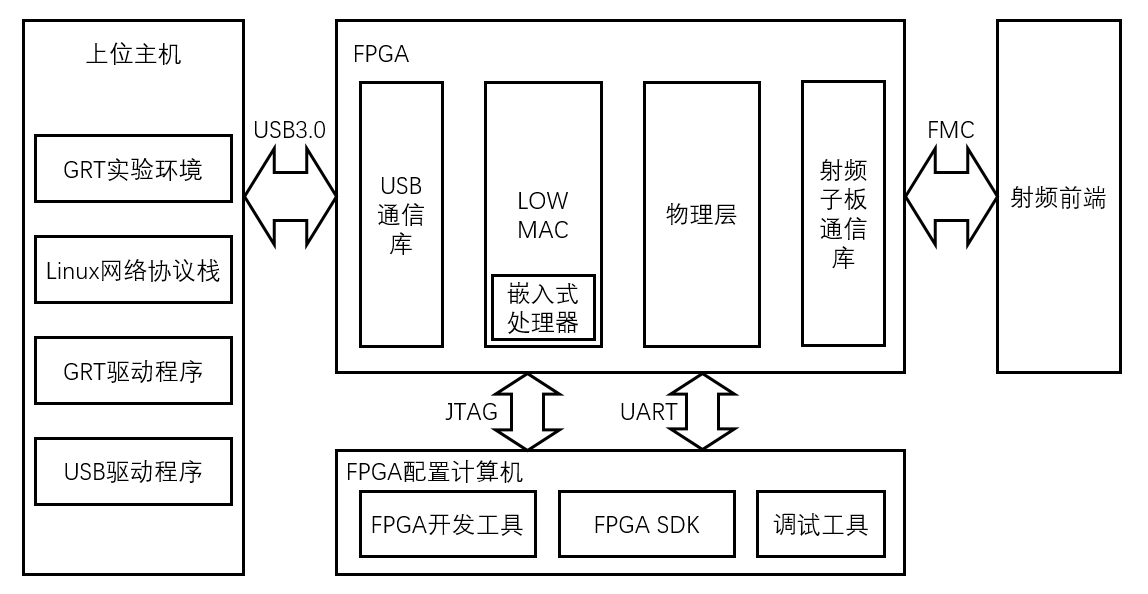
\includegraphics[width=1.0\textwidth]{img/GRT_overview.png}
			\caption{GRT2.0整体结构示意图}
			\label{fig:grt_overview}
		\end{figure}
	目前GRT2.0系统的FPGA部分使用的是Xilinx KC705开发板,后续版本也对Xilinx VC707进行了支持,
	上位主机使用的操作系统是Ubuntu14.04,
	FPGA配置计算机使用的开发工具是Vivado2015.2及其对应版本的SDK,
	射频前端使用的是Analog Device公司的EVAL-AD-FMCOMMS3-EBZ开发板\cite{fmcomms3}。

	值得一提的是,FPGA上的LOW MAC模块采用了软硬件协作的结构,
	将嵌入式处理器MicroBlaze\cite{microblaze}与硬件IP核\cite{xilinxip}结合,
	图\ref{fig:grt_lowmac}是LOW MAC模块软硬件协作的结构示意图,我参与了LOW MAC模块的搭建。
	硬件IP核是对完成特定功能的硬件逻辑的封装,
	嵌入式软件与硬件IP核结合的方式可以大大提高系统编程的灵活性。
	流程控制在嵌入式软件中实现,例如根据一帧的MAC地址进行分支处理,
	如果由硬件实现会非常繁琐,可读性和可扩展性差,
	数据通路和密集计算在硬件IP核中实现,例如发送端增加CRC校验位、接收端检测CRC是否匹配,
	硬件IP核可以每个时钟周期计算64bit的CRC,
	如果由软件实现会造成很高的延迟。
	在Vivado开发套件中,嵌入式处理器MicroBlaze与硬件IP核共同组织成block design\cite{xilinxblockdesign}的形式,具有图形化的开发界面。
	为了提高可编程性,本文在GRTSEC的设计中,也加入了软硬件协作的结构,第\ref{chap:grtsec_design}章会进行进一步介绍。

		\begin{figure}
			\centering
			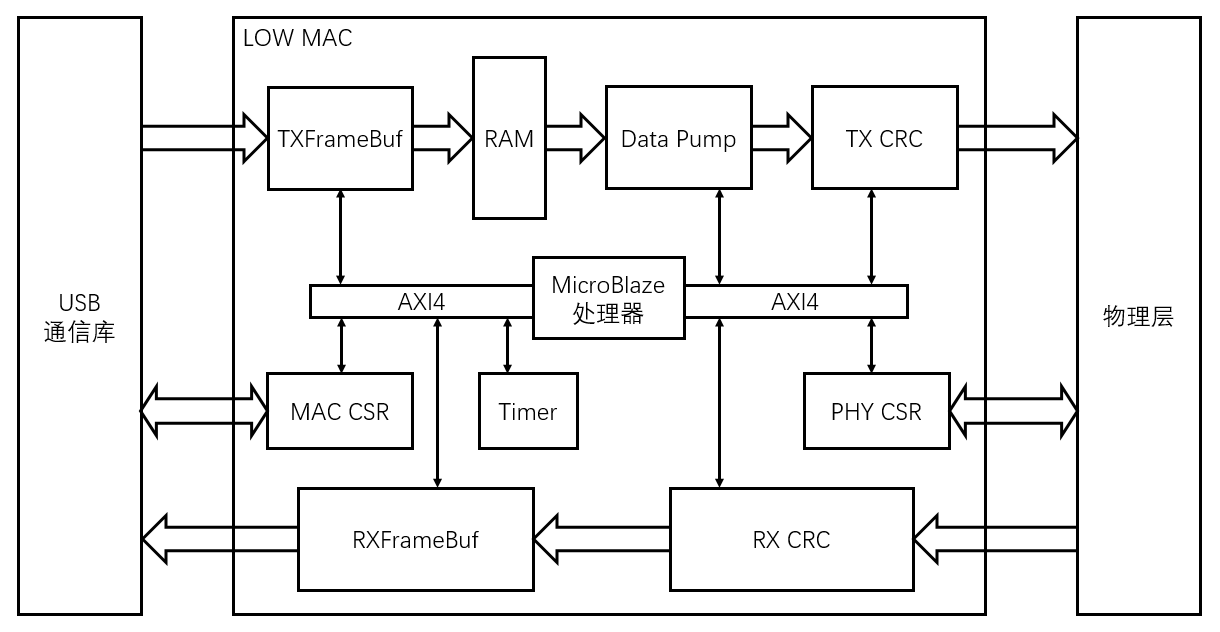
\includegraphics[width=1.0\textwidth]{img/GRT_lowmac.png}
			\caption{LOW MAC模块软硬件协同结构示意图}
			\label{fig:grt_lowmac}
		\end{figure}

	\section{射频通信库}\label{sec:grt2.0_rfd}
	射频前端是无线开放平台必备的组成部分,负责将数字基带信号转变为射频信号发送到空气中,
	以及接受空气中的射频信号转变为数字基带信号,射频前端的通信性能决定了无线平台的适用场景,
	对于WiFi无线验证平台,需要一个支持2.4GHz和5GHz中心频点、40MHz带宽的射频前端。
	作为一个提供给研究者的开放平台,除了考虑通信性能外,还要考虑价格,
	价格过高会让研究者望而却步。例如,OpenMili平台使用的射频前端\cite{mobicom16openmili}价格约11000美元,用于无线研究时价格过高。

	在GRT1.0系统中,我们选择使用USRP N210搭配XCVR2450子板\cite{usrpn210}作为射频前端,
	USRP N210价格是17000元,XCVR2450子板价格是4000元,属于可接受的范围。
	USRP的驱动是运行在Linux操作系统上的,称作UHD(USRP Hardware Driver),
	为了将FPGA开发板与射频前端相连,我们在FPGA上实现了USRP的硬件驱动,作为GRT1.0的射频通信库。
	这样的方式有以下几个缺点:
		\begin{itemize}
			\item XCVR2450子板最高支持25MHz带宽,无法达到802.11n协议要求的40MHz;
			\item USRP N210与FPGA开发板通过千兆以太网接口相连,
			以太网协议栈引入了不必要的延迟,经过GRT1.0射频通信库优化后的延迟也高达30ms以上,
			超过了802.11协议中要求的18ms的回复ACK的间隔,
			虽然可以与某些延迟要求宽松的商用设备实时通信,但系统的扩展性变得很差;
			\item 硬件实现USRP驱动的过程复杂,无法利用官方提供的软件驱动程序,也不方便驱动程序的升级换代;
			\item 不支持多天线MIMO(Multiple Input Multiple Output),MIMO技术是802.11n协议要求的技术。
		\end{itemize}

	以上缺点制约了无线平台的应用范围。

	在GRT2.0中,经过多方比较,我们选择使用性能更好、支持2x2 MIMO、具有通用接口的射频前端,
	Analog Device公司的EVAL-AD-FMCOMMS3-EBZ射频开发板\cite{fmcomms3},简称FMCOMMS3。
	FMCOMMS3的价格为6200元,射频芯片为Analog Device公司的AD9361,
	支持的中心频率范围是70MHz至6GHz,可以覆盖WiFi使用的2.4GHz和5GHz频段,
	带宽为200kHz至56MHz可调,支持802.11a协议要求的20MHz带宽、
	802.11b协议要求的18MHz带宽和802.11n协议要求的40MHz带宽,支持2x2 MIMO,
	通过高带宽的FMC接口(FPGA Mezzanine Card)\cite{wikifmc}与FPGA相连。
	虽然生产商提供了FPGA参考设计,但仍然无法直接与GRT系统集成,例如占用了过多的FPGA资源,没有提供上位主机配置射频参数的接口。
	射频通信库完成了GRT2.0系统与FMCOMMS3射频子板的对接。

	GRT2.0射频通信库的设计采用了嵌入式处理器与硬件IP核结合的方式。
	射频通信库软件部分所做的工作主要是对配置射频参数的接口进行封装,
	通过USB通信库与上位主机的驱动程序连接起来。
	由主机驱动程序配置的射频参数有中心频率和带宽,由射频通信库软件接口提供给主机驱动程序的是RSSI。

	射频通信库硬件部分对生产商提供的参考设计进行了较大的改造,体现在以下几点:
		\begin{itemize}
			\item 参考设计通过以太网与主机相连,通过HDMI与显示器相连,
			为降低FPGA资源使用率,射频通信库硬件部分去除对多种冗余接口的控制器,包括与主机相连的以太网接口控制器和以太网DMA控制器,
			与显示器相连的HDMI接口控制器,与板上LCD显示屏相连的LCD控制器,IIC接口控制器,只保留与FMC子板相连的FMC接口控制器;
			\item 参考设计将主机通过以太网发来的数据DMA到DDR3中,然后从DDR3中读取数据,
			经过AD9361 IP核转为时钟对齐的IQ两路数据,发送给FMCOMMS3子板,接收端与之方向相反,
			为降低数据传输延迟,射频通信库硬件部分去除收发数据读写DDR3的过程,直接转为FIFO接口与GRT系统的物理层模块相连;
			\item 参考设计中MicroBlaze配置级别高,性能好,
			为降低MicroBlaze占用的FPGA资源,射频通信库硬件部分简化了MicroBlaze的配置,
			提供支持射频通信库软件部分和LOW MAC软件部分的最小集合。
		\end{itemize}

	下面分别介绍射频通信库的数据通路的硬件接口和配置的嵌入式软件接口。
	在硬件设计中,射频通信库将AD9361 IP核输出的IQ两路数据转化为标准的FIFO接口,提供给物理层,并通过异步FIFO的方式完成时钟域转换。
	射频侧的时钟和复位信号由AD9361 IP核提供,这个时钟是随采样率变化的;物理层侧的时钟和复位信号由物理层提供。
	硬件接口以简单明了为目标,
	射频通信库与物理层之间的接口定义如下:
	\begin{lstlisting}[language={Verilog}]
module fmc_iface
(
input fmc_clk,
input fmc_rst,
input PHY_TX_clk,
input PHY_RX_clk,
input PHY_rst,
output PHY2RF_FIFO_prog_full,
input PHY2RF_FIFO_wr_en,
input [31:0] PHY2RF_FIFO_din,
input RF2PHY_FIFO_rd_en,
output [31:0] RF2PHY_FIFO_dout,
output RF2PHY_FIFO_empty,
output RF2PHY_FIFO_almost_empty
);
	\end{lstlisting}

	射频通信库在嵌入式软件端提供了配置射频参数接口。
	包括初始化射频子板,对射频子板的ADC、DAC、滤波器等初始化配置,设置中心频率、采样率、发送增益等射频参数。
	中心频率的单位是MHz,比如WiFi标准频段的信道1为2412MHz。
	采样率的单位为Sps(Samples per seconds),比如802.11a/g的采样率为20000000Sps,802.11n需要40000000Sps的模式。
	发送增益以衰减的形式表示,单位是mdb,即db的千分之一,设置为0时表示无衰减,1000时为衰减为十分之一。
	射频通信库提供的软件配置接口如下:
	\begin{lstlisting}[language={C}]
int fmc_main(void);
void set_rx_samp_freq(double* param, char param_no);
void set_tx_samp_freq(double* param, char param_no);
void set_rx_lo_freq(double* param, char param_no);
void set_tx_lo_freq(double* param, char param_no);
void set_tx1_attenuation(double* param, char param_no);
	\end{lstlisting}

	\section{工程自动化脚本}\label{sec:grt2.0_script}
	TCL脚本在FPGA的开发过程中有着广泛的运用\cite{xilinxtcl},从模块间引脚的连接、工程文件的组织,
	到调试信息的导出、自动执行工作流程,TCL脚本大大提高了FPGA开发的效率。
	为了将GRT2.0系统开源给研究者,我们提供了可以自动搭建工程项目的TCL脚本,
	实现了从源代码、资源文件到最终二进制文件的自动化过程。
	TCL脚本的使用是从GRT1.0到GRT2.0的一个重要改进。

	GRT2.0系统提供的工程自动化TCL脚本完成了以下过程:
		\begin{itemize}
			\item 对GRT2.0提供的完成特定功能的硬件逻辑封装成IP核;
			\item 生成block design中的各个模块和输入输出端口,完成模块间、端口间互相的连线;
			\item 生成和配置嵌入式处理器MicroBlaze及其附属的总线控制器,对总线地址进行分配;
			\item 对Xilinx提供的IP核进行配置,并添加到工程中,主要是各种不同类型的FIFO、时钟生成器、RAM、DDR3控制器等;
			\item 添加GRT2.0的资源文件,有约束文件、三角函数数据文件、OFDM导频数据文件等;
			\item 执行工作流程,设置流程策略,工作流程有综合(Synthesis)、布局(Place)、布线(Route)、生成二进制文件(Generate Bitstream)等。
		\end{itemize}

	通过执行工程自动化TCL脚本,用户可以利用手中的开发板和开源的GRT2.0代码,生成可以烧写FPGA的二进制文件,
	再结合我们提供的上位主机的驱动程序,用户便自行搭建GRT2.0系统完成。

	\section{用于安全研究时的不足}\label{sec:grt2.0_drawback}
	基于GRT2.0系统进行开发,可以满足设计目标中的与商用网卡实时通信,以及与上层网络协议栈连接,
	但在其他方面存在不足,尤其是无法获取物理层WiFi安全研究所需要的物理层信息。
	GRT2.0系统中物理层接收端的设计目标是消除接收信号的偏差,还原出发送信号,
	频偏纠正、相位纠正、信道均衡、Viterbi解码等过程都是为了完成这个目标,
	然而在物理层WiFi安全的研究中,接收信号的偏差有其背后的物理含义,常常被拿来做研究,
	但GRT2.0的系统框架不支持这些信息的提取。
	具体来说,用于安全研究时的不足包括以下几点。
		\begin{itemize}
			\item 物理层由单一的硬件逻辑实现,可编程性还不够高;
			\item 未提供方便获取CSI、RSSI的接口,CSI和RSSI是安全研究常用的指标;
			\item 在接收端数据处理过程中消除了信号偏差,而这些偏差在安全研究中常常被用到,例如频偏;
			\item 不支持软硬件数据处理模块替换的能力;
			\item 缺乏物理层编程的使用样例。
		\end{itemize}

	在第\ref{chap:grtsec_design}章将针对以上问题加以改进,
	介绍适用于物理层WiFi安全研究的验证平台GRTSEC的设计与实现。

	\section{本章小结}\label{sec:grt2.0_summary}
	本节对支持物理层WiFi安全研究的验证平台GRTSEC的前期工作GRT2.0系统进行了介绍,
	GRT2.0系统硬件上包括上位主机、FPGA、射频前端、配置计算机,
	由物理层模块、LOW MAC模块、射频通信库、USB通信库等模块组成。
	GRT2.0系统可以满足本文设计目标中的与商用网卡实时通信,以及与上层网络协议栈连接,
	但在获取物理层信息、物理层编程性、软硬件模块替换等方面存在不足。
	另外,本节展开介绍了本人在GRT2.0系统中完成的工作,主要负责完成的射频通信库、工程自动化脚本,
	参与完成的LOW MAC软硬件协作设计。

	% Copyright (c) 2008-2009 solvethis
% Copyright (c) 2010-2011 Casper Ti. Vector
% Public domain.

\chapter{验证平台使用样例设计}
	本章会通过两个实际的物理层WiFi安全研究的样例,进一步说明GRTSEC平台的使用场景和方法,
	同时,用户也可以基于这些使用样例开展自己的研究。
	在\ref{sec:demo_fake_wifi}节会介绍如何使用GRTSEC搭建伪装WiFi,并用伪装WiFi发起钓鱼攻击,获取用户的敏感信息,
	在\ref{sec:demo_phy_auth}节会提出一种利用利用硬件指纹技术对不同WiFi设备进行识别的方法。

	\section{搭建伪装AP}\label{sec:demo_fake_wifi}
	身份伪装是很多WiFi攻击的前提和基础,比如DoS攻击、会话劫持、中间人攻击、数据篡改、窃听等\cite{ieeewc10}。
	针对身份伪装的安全研究需要先搭建伪装AP,本节设计了搭建伪装AP的样例,并用伪装AP发起钓鱼攻击,获取用户的敏感信息,

		\subsection{样例背景}
		在北京大学,计算中心为全校师生员工提供了无线校园WiFi,名字是WirelessPKU,遍布教学楼、实验室、食堂等场所。
		WirelessPKU是无密码的开放WiFi,用户连接到WirelessPKU后,首先跳转到一个认证网页,输入网关的账号、密码进行登录,
		登录后才可以继续上网。对于学生来说,网关账号、密码同时也是其他校园网页登录的账号、密码,
		包括信息登记、成绩查询、选课申请等都使用同一套认证系统。
		假如密码泄露会造成巨大的损失,轻则已选的课程被退掉或者成绩泄露,重则学籍信息被篡改,无法毕业。
		在本节,我们将利用GRTSEC搭建AP,伪装成WirelessPKU,并制作一个钓鱼认证网页,用来盗取统一认证账号。

		\subsection{场景设计}
		真实WirelessPKU的AP与伪装AP的分布场景如图\ref{fig:demo_fake_wifi_scenary}所示,
		这张图真实地模拟了北京大学理科五号楼五楼的AP分布,其中AP1、AP2、AP3是北京大学计算中心布置的WirelessPKU的AP,
		GRTSEC摆放在房间1中。假设AP1、AP2、AP3的MAC地址是$MA_1$、$MA_2$、$MA_3$。
		房间1内有个用户,我们称他为小明,在GRTSEC发起伪装之前,小明可以看到信号较强的AP1和信号弱一些的AP2,看不到远处的AP3。
		为了让小明能够连接上GRTSEC,我们将GRTSEC的SSID设置为WirelessPKU,将MAC地址设置为$MA_3$,
		即使小明用MAC地址的白名单来分辨伪装AP也是无法识别的。小明连接上GRTSEC搭建的AP后,会先看到钓鱼认证网页,
		习惯了上网认证的小明会毫无戒心的输入自己的统一认证账号和密码。

		此样例旨在说明设计目标中的两点:可与商用802.11设备实时通信,在这里是与小明的手机相连;
		% 支持自定义数据处理流程,在这里是监听特定包并发送干扰信号;
		可与上层网络协议栈连接,在这里是与应用层的钓鱼认证网页相连。

			\begin{figure}
				\centering
				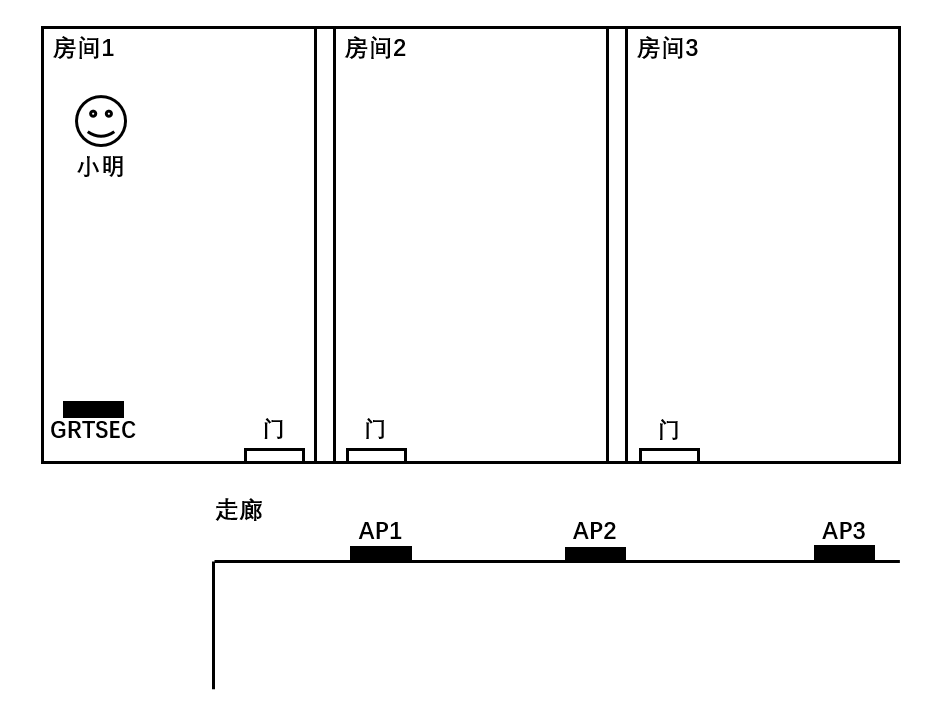
\includegraphics[width=0.7\textwidth]{img/demo_fake_wifi_scenary.png}
				\caption{伪装AP与真实AP分布场景图}
				\label{fig:demo_fake_wifi_scenary}
			\end{figure}

		\subsection{样例实现}
		首先,在上位主机上搭建钓鱼认证网页,钓鱼网页参考了本组张高瀚同学做的网页\cite{zgh17wifi},
		然后,修改主机的网络配置,使网络请求都转跳到钓鱼认证网页,
		最后,将GRTSEC运行在AP模式,等待进入房间1的用户连接。

	\section{利用物理层信息识别不同WiFi设备}\label{sec:demo_phy_auth}
	在802.11协议中,WiFi身份的标识是MAC地址,然而MAC地址非常容易伪装,利用笔记本电脑,
	或者一部root过的安卓手机,搭配一些软件工具,就可以任意修改自己的MAC地址\cite{NetworkSecurity11hacking}。
	在本节,我们提出一种利用物理层信息识别WiFi设备的方法,具体来说,使用物理层信息中的频偏和时钟偏移,识别不同的WiFi设备硬件,
	弥补仅靠MAC地址进行识别的缺陷。

		\subsection{样例背景}\label{subsec:demo_trusted_sta}
		一些用户家里的WiFi偶然被邻居知道了密码,又不想修改密码使自己的全部设备重新输入一次,我们假设这样的一个用户叫小明。
		为了防止邻居的“蹭网”,小明会对路由器进行设置,只允许特定MAC地址的设备连接,目前很多路由器支持这种模式。
		但是,不怀好意的邻居可以监听到小明设备的MAC地址,将自己的设备伪装成小明的设备骗过路由器,继续进行蹭网。
		小明希望做的是对自己的设备进行信任而不是对MAC地址进行信任,在本节,我们利用GRTSEC从接收到的包中提取频偏和时钟偏移,
		生成与WiFi设备对应的硬件指纹,这样小明可以在路由器端选择对特定硬件指纹进行信任,防止邻居继续蹭网。

		本样例主要关注对不同WiFi设备的识别和区分,并不针对无线路由器识别用户设备,实际上这种方法是通用的,
		可用于AP识别STA,可用于识别\ref{sec:demo_fake_wifi}节提出的伪装AP,也可用于STA之间的互相识别。

		\subsection{场景设计}
		我们对AP模式和STA模式的设备进行测试,设计了以下场景。
			\begin{itemize}
				\item 区别不同的STA,使手机和笔记本电脑工作在STA模式,用GRTSEC对这些设备进行区分,
				应用场景是\ref{subsec:demo_trusted_sta}小节提到的防邻居“蹭网”;
				\item 区别不同的AP,在同一地点存在多个同SSID的AP,用GRTSEC进行区分,
				应用场景是识别\ref{sec:demo_fake_wifi}节提出的伪装AP。
			\end{itemize}

		\subsection{样例实现}
		首先,我们利用GRTSEC监听周边WiFi设备发出的包,记录物理层信息,切换多个频道进行记录,
		区别不同的STA时,由于STA不会定时发送beacon包,我们无法获得时钟偏移,只能得到频偏,因此区别不同STA的场景采集的物理层信息是频偏,
		而其他两种场景采集的物理层信息是频偏和时钟偏移。
		然后,我们将记录到的前半部分数据作为训练集,利用KNN(K-nearest neighbors)算法进行建模。
		最后,我们将记录到的后半部分数据作为测试集,用训练好的模型进行区分。
		训练和测试代码都由Python实现。

	% Copyright (c) 2008-2009 solvethis
% Copyright (c) 2010-2011 Casper Ti. Vector
% Public domain.

\chapter{性能测试与评估}
本章将对支持物理层WiFi安全研究的验证平台GRTSEC进行评估。
首先在\ref{sec:envaluation_env_setup}节介绍测试环境,介绍开发板型号、开发套件版本号等,
其次在\ref{sec:envaluation_performance}节对验证平台的性能进行测试,
然后在\ref{sec:envaluation_demo}节对第五章提出的使用样例进行测试,
最后在\ref{sec:envaluation_summary}节对本章进行总结。

  \section{测试环境}\label{sec:envaluation_env_setup}
  在第四章我们介绍了GRTSEC的前期工作GRT2.0的组成部分,GRTSEC与GRT2.0的组成部分相同,但具体测试环境略有不同。
  在GRTSEC中,我们使用的上位主机是一台支持USB3.0接口、运行有Ubuntu14.04操作系统的计算机,
  FPGA是一块Xilinx VC707板卡\cite{xilinxvc707},
  配置计算机是任意一台支持Xilinx Vivado开发套件的计算机,Windows系统或Linux系统均可,
  射频前端是Analog Device公司的EVAL-AD-FMCOMMS3-EBZ开发板\cite{fmcomms3}。
  FPGA开发工具我们使用的是Xilinx Vivado 2015.2,FPGA嵌入式软件开发工具是Xilinx SDK 2015.2。

  \section{平台性能测试}\label{sec:envaluation_performance}
  在本节我们介绍GRTSEC的性能,GRT2.0的性能可参考\cite{cjh16grt},如吞吐率、延迟等,
  本文主要对GRTSEC相对于GRT2.0的扩展性能进行测试。

  首先是FPGA的资源占用率,GRT2.0的资源占有率见表\ref{tab:envaluate_grt2.0_resource},
  增加GRTSEC的扩展后,资源占用率见表\ref{tab:envaluate_grtsec_resource}。
    \begin{table}[!hbp]
    \centering
    \caption{GRT2.0在VC707开发板上的资源占用率}
    \label{tab:envaluate_grt2.0_resource}
      \begin{tabular}{|l|l|l|l|} \hline
      资源 & 已使用 & 总数 & 占用率 \\ \hline
      Flip-Flop & 76781 & 607200 & 12.65 \\ \hline
      LUT & 98657 & 303600 & 32.50 \\ \hline
      Memory LUT & 4551 & 130800 & 3.48 \\ \hline
      I/O & 224 & 700 & 32.00 \\ \hline
      BRAM & 319 & 1030 & 30.97 \\ \hline
      DSP48 & 294 & 2800 & 10.50 \\ \hline
      BUFG & 17 & 32 & 53.12 \\ \hline
      MMCM & 4 & 14 & 28.57 \\ \hline
      PLL & 1 & 14 & 7.14 \\ \hline
      \end{tabular}
    \end{table}
    \begin{table}[!hbp]
    \centering
    \caption{GRTSEC在VC707开发板上的资源占用率}
    \label{tab:envaluate_grtsec_resource}
      \begin{tabular}{|l|l|l|l|} \hline
      资源 & 已使用 & 总数 & 占用率 \% \\ \hline
      Flip-Flop & 79564 & 607200 & 13.10 \\ \hline
      LUT & 95761 & 303600 & 31.54 \\ \hline
      Memory LUT & 4058 & 130800 & 3.10 \\ \hline
      I/O & 224 & 700 & 32.00 \\ \hline
      BRAM & 263 & 1030 & 25.53 \\ \hline
      DSP48 & 303 & 2800 & 10.82 \\ \hline
      BUFG & 14 & 32 & 43.75 \\ \hline
      MMCM & 4 & 14 & 28.57 \\ \hline
      PLL & 1 & 14 & 7.14 \\ \hline
      \end{tabular}
    \end{table}

  我们可以看到,资源使用率没有增加太多,因为GRTSEC主要利用原有信号进行物理层信息的提取,
  而且采用多级寄存器缓存技术进行帧对齐,而不是用FIFO进行缓存,节约了存储空间。

  然后是嵌入式软件代码的性能,主要体现在传输延迟上。从收到一帧到回复ACK的时间间隔,是最关键的延迟指标,
  如果延迟太高,会大大影响传输性能,留给用户可编程的空间会降低。
  GRTSEC相对GRT2.0增加了读取物理层信息的过程,本节对GRT2.0和GRTSEC在这方面的性能进行对比,
  性能结果见表\ref{tab:envaluate_grtsec_latency}。
  (此处需要搭建两台GRT,互相收发数据测试延迟)
  \begin{table}[!hbp]
  \centering
  \caption{GRTSEC与GRT2.0的延迟性能对比表}
  \label{tab:envaluate_grtsec_latency}
    \begin{tabular}{|l|l|l|l|} \hline
    帧长度 & 调制方式 & GRT2.0延迟 & GRTSEC延迟 \\ \hline
    20 & ?? & ?? & ?? \\ \hline
    100 & ?? & ?? & ?? \\ \hline
    1500 & ?? & ?? & ?? \\ \hline
    4095 & ?? & ?? & ?? \\ \hline
    \end{tabular}
  \end{table}

  我们可以看到,延迟没有增加太多,因为经过精心设计的硬件逻辑,可以保证在软件读取之前将物理层信息准备好。

  最后是读取物理层信息的有效性,选用真实的802.11设备进行测试,地点是北京大学理科五号楼五楼。
  我们在2.4GHz频段的最常用1号信道以及5GHz频段的149信道,对该频段挑选最活跃3个真实设备的进行监听,
  记录频偏、CSI、RSSI、调制方式等物理层信息,绘制成以下图表。

  (此处共7张图,频偏、CSI、RSSI各附上两张图,2.4GHz和5GHz,调制方式附上一张图。
  频偏的图是设备频偏变化图,横轴是时间,纵轴是频偏,画3条线。
  CSI的图是三维的,X轴是时间,Z轴是CSI大小,Y轴是子信道,画3个曲面。
  RSSI与频偏类似。调制方式是分布折线图,6个设备放在一张图里,横轴是调制方式,纵轴是所占比例。)

  我们可以看到,频偏值随时间的变化不大,随设备的变化大,CSI和RSSI随时间变化大。

  \section{样例测试}\label{sec:envaluation_demo}
  在本节对第五章提出的使用样例进行测试。
    \subsection{搭建伪装AP}
    搭建伪装AP主要测试其有效性。
    如图\ref{fig:envaluation_fake_ap}所示,我们利用GRTSEC搭建伪装AP,可以被一部手机连接,手机任意输入一个网址可以跳转到钓鱼页面。
    (下图要换掉,用GRT搭建,修改个SSID,重新截图)
  		\begin{figure}[H]
  			\centering
  			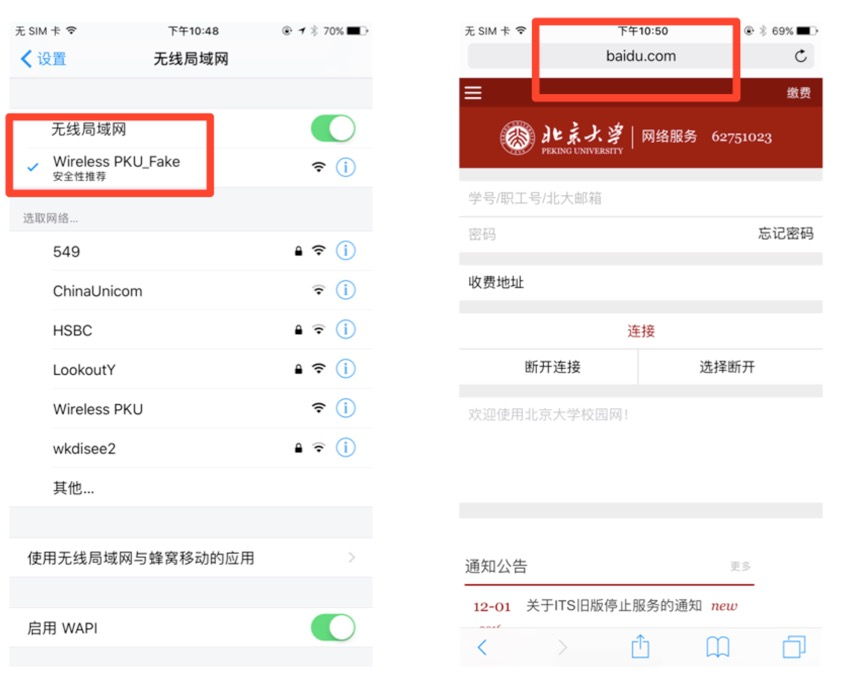
\includegraphics[width=0.5\textwidth]{img/WirelessPKU_fake_1.jpg}
  			\caption{伪装AP与钓鱼认证网页}
  			\label{fig:envaluation_fake_ap}
  		\end{figure}

    我们可以看到,用户手机真实连上了GRTSEC搭建的伪装AP,说明GRTSEC可与商用设备实时通信,
    用户手机看到了钓鱼认证网页,说明GRTSEC兼容上层网络应用。

    \subsection{利用物理层信息识别不同WiFi设备}
    \ref{sec:demo_phy_auth}中提到,我们对三种情况进行测试,区别不同的STA、区别不同地点的AP、区别同一地点的不同AP。

    首先是区别不同的STA,我们对三台设备进行监听,记录频偏值,采用KNN算法,
    测试结果如表\ref{tab:envaluate_identify_sta}所示。
      \begin{table}[!hbp]
      \centering
      \caption{利用物理层信息识别不同的STA}
      \label{tab:envaluate_identify_sta}
        \begin{tabular}{|l|l|l|l|l|} \hline
        设备 & 训练集组数 & 测试集组数 & 正确率 & 误判率 \\ \hline
        华为手机 & ?? & ?? & ?? & ?? \\ \hline
        OPPO手机 & ?? & ?? & ?? & ?? \\ \hline
        三星笔记本电脑 & ?? & ?? & ?? & ?? \\ \hline
        \end{tabular}
      \end{table}

    然后是区别不同的AP,我们对三个WirelessPKU的AP进行监听,以频偏值和时钟偏移为特征进行训练和测试,
    测试结果如表\ref{tab:envaluate_identify_ap}所示。
      \begin{table}[!hbp]
      \centering
      \caption{利用物理层信息识别不同地点的AP}
      \label{tab:envaluate_identify_ap}
        \begin{tabular}{|l|l|l|l|l|} \hline
        设备 & 训练集组数 & 测试集组数 & 正确率 & 误判率 \\ \hline
        WirelessPKU AP1 & ?? & ?? & ?? & ?? \\ \hline
        WirelessPKU AP2 & ?? & ?? & ?? & ?? \\ \hline
        WirelessPKU AP3 & ?? & ?? & ?? & ?? \\ \hline
        \end{tabular}
      \end{table}

    以上两个实验可以看到,通过物理层信息频偏和时钟偏移对不同设备进行识别,正确率较高,
    这种方法可以在多种场景下进行应用。

  \section{总结}\label{sec:envaluation_summary}
  本章对支持物理层WiFi安全研究的验证平台GRTSEC进行了评估,实验表明GRTSEC在没有明显资源占用和性能降低的情况下,
  支持多种物理层信息的提取,通过使用样例说明了支持物理层WiFi安全研究。

	% 结论。
	% Copyright (c) 2008-2009 solvethis
% Copyright (c) 2010-2011 Casper Ti. Vector
% Public domain.

\chapter{结论与展望}
本章将在\ref{sec:conclusion}进行总结,在\ref{sec:future_work}进行未来工作展望。

  \section{总结}\label{sec:conclusion}
  本文首先对物理层WiFi安全的研究进行了深入的调研,总结了物理层WiFi安全研究对无线验证平台的需求,
  指出了现有无线验证平台的不足,提出了验证平台的设计目标。

  本文提出一种新型的支持物理层WiFi安全研究的验证平台GRTSEC,并且在北京大学可重构体系结构课题小组提出的GRT2.0系统的基础上加以实现。
  针对GRT2.0在物理层WiFi安全研究方面的几点不足,GRTSEC进行了相应的改进。

  为了更好的说明GRTSEC在物理层WiFi安全研究方面的优势,本文设计并实现了多个使用样例,
  实验表现使用样例在设备认证等方面改进了现有的WiFi安全机制,研究者也可以基于使用样例进行更深入的研究或开发。

  \section{未来工作展望}\label{sec:future_work}
  GRTSEC作为GRT2.0系统的扩展,一些特性将会在下一代GRT系统GRT3.0中加以应用,比如物理层信息从硬件逻辑到嵌入式软件的通道,
  因此未来的一项工作是将GRTSEC的特性合并到GRT主线的开发中。

  另外,我们发现开发硬件时调试困难,开发周期较长,研究者常常受困于安全算法的硬件实现,
  Xilinx开发套件提供的HLS(High-Level Synthesis,高层次综合)\cite{xilinxhls}工具可以有效地降低开发难度,提供开发效率。
  目前GRTSEC的框架是支持HLS的,将来希望针对HLS进行进一步地优化,比如提供适用于HLS的硬件模块接口。

  其次,在软件开发方面,我们在嵌入式软件中应用了Xilinx提供的xilkernal,这是一个简易的操作系统,提供pthread等多线程库,
  但是Xilinx在SDK 2017.1及之后的版本舍弃了xilkernal,转而支持Free RTOS,因此将来的一项工作是将GRTSEC的软件代码移植到新的嵌入式操作系统上。

  最后,根据GRT的新特性,GRTSEC也会提取更多的适用于安全研究的物理层信息,比如与多天线相关的信息。


	\begin{appendix}
		% 参考文献。
		\bibliography{ref/thesis}
		% 各附录。
		% Copyright (c) 2008-2009 solvethis
% Copyright (c) 2010-2011 Casper Ti. Vector
% Public domain.

\chapter{攻读硕士学位期间发表的论文及专利}
\raggedbottom % 避免某些奇怪的“Underfull \vbox”警告。
	\begin{description}
		\subsection*{已授权专利}
		\item{[1]} 王韬、\textbf{李晓光}、吴浩洋、吕松武,“一种基于FPGA的无线电光纤连接接口通信库及其实现方法”,
		授权日:2017年3月28日,专利号:201510239058.6
		\subsection*{已申请专利}
		\item{[2]} 王韬、\textbf{李晓光}、吴浩洋、吕松武,“一种利用物理层信息识别伪装WiFi的方法和系统”,
		申请日:2017年3月21日,申请号:201710169111.9
		\subsection*{已发表论文}
		\item{[3]} Tao Wang, Guangyu Sun, Jiahua Chen, Jian Gong, Haoyang Wu, \textbf{Xiaoguang Li}, Songwu Lu, and Jason Cong, "GRT: a Reconfigurable SDR Platform with High Performance and Usability," ACM SIGARCH Computer Architecture News (CAN), Vol. 42, No. 4, pp. 51-56, September 2014

		\item{[4]} Jiahua Chen, Tao Wang, Haoyang Wu, Jian Gong, \textbf{Xiaoguang Li}, Yang Hu, Gaohan Zhang, Zhiwei Li, Junrui Yang, and Songwu Lu, "A High-performance and High-programmability Reconfigurable Wireless Development Platform (Demonstration Paper)," in Proceedings of the 2014 International Conference on Field-Programmable Technology (ICFPT 2014), December 10-12, 2014, Shanghai, China, pp. 350-353.

		\item{[5]} Haoyang Wu, Tao Wang, Zhiwei Li, Boyan Ding, \textbf{Xiaoguang Li}, Tianfu Jiang, Jun Liu, and Songwu Lu, "GRT 2.0: An FPGA-based SDR Platform for Cognitive Radio Networks (Abstract Only)," in Proceedings of ACM/SIGDA International Symposium on Field-Programmable Gate Arrays (FPGA 2017), February 22-24, 2017, Monterey, CA, USA, pp. 294-295.

		\item{[6]} 吴浩洋、王韬、陈佳华、龚健、\textbf{李晓光}、张高瀚、吕松武, "GRT:高性能可定制无线网络底层软硬件开放平台," 电子科技大学学报, Vol. 44, No. 1, pp. 123-128, 2015年1月.

		\item{[7]} Yang Tian, Kaigui Bian, Guobin Shen, Xiaochen Liu, \textbf{Xiaoguang Li}, Thomas Moscibroda, "Contextual-code: Simplifying information pulling from targeted sources in physical world," in Computer Communications (INFOCOM), 2015 IEEE Conference on. IEEE, 2015: 2245-2253.
		\subsection*{已投稿论文}
		\item{[8]} Haoyang Wu, Tao Wang, Zhiwei Li, Boyan Ding, \textbf{Xiaoguang Li}, "The Tick Programmable Low-Latency SDR System," in Computer Communications (INFOCOM), 2017 IEEE Conference on.

	\end{description}

\flushbottom % 取消 \raggedbottom 的作用。

	\end{appendix}

	% 以下为正文之后的部分。
	\backmatter

	% 致谢。
	% Copyright (c) 2008-2009 solvethis
% Copyright (c) 2010-2011 Casper Ti. Vector
% Public domain.

\chapter{致谢}
时光荏苒,岁月如梭,三年的硕士时光很快就要过去了,搭环境、写代码、调参数、读论文的场景还历历在目。
三年来我经历了挫折与历练,也经历了收获与喜悦,感谢导师、同学、朋友、家人的陪伴,在我困难时给予我支持,在我快乐时共同分享,
这些都将是我宝贵的财富,我会一直铭记。

首先,我要感谢我的导师王韬老师。王老师是我从大三到研究生期间最重要的引路人,不仅在学业、科研、工作上给予我启迪与帮助,还在做人做事上起到了表率作用。
王老师平易近人、身体力行,我还记得大四时王老师陪伴我们调试代码,教给我调试技巧,其兢兢业业的工作态度是激励我踏实勤奋的重要动力。
后来课题组日渐壮大,年轻学生不断加入,王老师告诉我们一个人能力再强,也无法独立完成大的工作,只有将学会的东西分享出去,互相学习、互相促进,
在一个团队中协力合作,凝聚力量,才能完成更大的工作。我学会了分享与学习,学会了相信同伴,这在我后来的科研和工作中受益匪浅。
王老师教育我们坚持手中的工作,勤奋努力,哪怕短时间内无法获得成效,长期的积累会带来坚实的收获,几位师兄师姐厚积薄发的科研和工作经历印证了这一点。
努力不一定得到回报,但不努力肯定没有回报,坚持努力总会获得回报。
王老师学识渊博,还不忘与时俱进、坚持读书与学习。王老师最初在体系结构方面颇有建树,这些年来又在软件工程、项目管理、人工智能等领域拓展自己的能力,
与学生一起重学概率论、研究小样本学习,给我留下很深的印象,学业的结束不代表学习的结束,我们只有坚持吸取养分,结合温故知新,才能跟上时代的步伐,与时俱进。
老师的悉心栽培恩重如山,非区区百字可以言表,我当铭记于心,砥砺前行。

然后,我要感谢吕松武老师。吕老师也指导了我五年的时间,虽然长期在美国,每年只回国数次,但每次都能为我们带来行业最新的进展,带来国际化的视野。
吕老师让我们看到了国际上最优秀的学生是如何学习和工作的,告诉我们怎样成为最优秀的学生。
除此之外,吕老师在生活和求职上也给予我巨大的帮助,与王老师一样,不仅是我学习和科研的导师,更是教给了我做人的道理,是我人生的导师。
我要感谢刘君老师,刘老师雷厉风行的做事风格为组里带来了执行力,并且在生活上给予我和我的妻子帮助,是我的良师益友。

此外,我要感谢我们实验室高能效计算与应用中心的同学们,我的工作离不开你们的帮助。
感谢龚健师兄,你的严谨认真的态度为组里的师弟师妹们带来表率,你的代码结构清晰、表意明确,论文严谨细致,是我们课题组的开拓者。
感谢陈佳华师姐,你工作勤奋、勇于探索、乐于创新,是组里的中坚力量,毕业后也不忘回报课题组。
感谢吴浩洋师兄,你是组里唯一的博士,是我的毕业论文最重要的协作者,你的沉稳、低调、务实帮助组里完成很多困难的工作,是真正的攻坚人。
感谢李志伟师弟和丁博岩师弟,在我做毕业设计的过程中给予我巨大的帮助和启发,是值得信任的伙伴。
感谢同级同学张高瀚、严磊,在一起做毕设的过程中是我站在同一战线的战友,讨论进展、相互支持。
感谢蒋天夫师弟、吴涵师妹、樊乃嘉师妹,你们为组里带来了活力和生机。
感谢同实验室的张宸师兄、王鹏师兄、魏学超师兄、王硕师兄、张炜其、姜双、王丰、肖倾城等,我在实验室得到了你们的不少帮助。

最后,我要感谢我的家人。谢谢妈妈在生活上的支持,多年来独自带我成长不易,养育之恩,寸心难报。
谢谢我的妻子周易,从相识到相爱到步入婚姻殿堂,一路上陪伴我共乘风雨、共享欢乐。

	% 原创性声明和使用授权说明。
	% Copyright (c) 2008-2009 solvethis
% Copyright (c) 2010-2011 Casper Ti. Vector
% All rights reserved.
%
% Redistribution and use in source and binary forms, with or without
% modification, are permitted provided that the following conditions are
% met:
%
% * Redistributions of source code must retain the above copyright notice,
%   this list of conditions and the following disclaimer.
% * Redistributions in binary form must reproduce the above copyright
%   notice, this list of conditions and the following disclaimer in the
%   documentation and/or other materials provided with the distribution.
% * Neither the name of Peking University nor the names of its contributors
%   may be used to endorse or promote products derived from this software
%   without specific prior written permission.
%
% THIS SOFTWARE IS PROVIDED BY THE COPYRIGHT HOLDERS AND CONTRIBUTORS "AS
% IS" AND ANY EXPRESS OR IMPLIED WARRANTIES, INCLUDING, BUT NOT LIMITED TO,
% THE IMPLIED WARRANTIES OF MERCHANTABILITY AND FITNESS FOR A PARTICULAR
% PURPOSE ARE DISCLAIMED. IN NO EVENT SHALL THE COPYRIGHT HOLDER OR
% CONTRIBUTORS BE LIABLE FOR ANY DIRECT, INDIRECT, INCIDENTAL, SPECIAL,
% EXEMPLARY, OR CONSEQUENTIAL DAMAGES (INCLUDING, BUT NOT LIMITED TO,
% PROCUREMENT OF SUBSTITUTE GOODS OR SERVICES; LOSS OF USE, DATA, OR
% PROFITS; OR BUSINESS INTERRUPTION) HOWEVER CAUSED AND ON ANY THEORY OF
% LIABILITY, WHETHER IN CONTRACT, STRICT LIABILITY, OR TORT (INCLUDING
% NEGLIGENCE OR OTHERWISE) ARISING IN ANY WAY OUT OF THE USE OF THIS
% SOFTWARE, EVEN IF ADVISED OF THE POSSIBILITY OF SUCH DAMAGE.

% 原创性声明和使用授权说明页不需要装订到论文中,故不显示页码。
\cleardoublepage\pagestyle{empty}
{
	\linespread{1.5}\selectfont
	\section*{北京大学学位论文原创性声明和使用授权说明}

	\vfill
	\section*{原创性声明}

	本人郑重声明:
	所呈交的学位论文,是本人在导师的指导下,独立进行研究工作所取得的成果。
	除文中已经注明引用的内容外,
	本论文不含任何其他个人或集体已经发表或撰写过的作品或成果。
	对本文的研究做出重要贡献的个人和集体,均已在文中以明确方式标明。
	本声明的法律结果由本人承担。
	\vspace{2.5em}\par
	\rightline
	{%
		论文作者签名:\hspace{5em}%
		日期:\hspace{2em}年\hspace{2em}月\hspace{2em}日%
	}

	\vfill
	\section*{学位论文使用授权说明}
	\vspace{-1em}\par
	\centerline{\zihao{-4}(必须装订在提交学校图书馆的印刷本)}
	\vspace{1em}\par

	本人完全了解北京大学关于收集、保存、使用学位论文的规定,即:
	\begin{itemize}
		\item 按照学校要求提交学位论文的印刷本和电子版本;
		\item 学校有权保存学位论文的印刷本和电子版,
			并提供目录检索与阅览服务,在校园网上提供服务;
		\item 学校可以采用影印、缩印、数字化或其它复制手段保存论文;
		\item 因某种特殊原因需要延迟发布学位论文电子版,
			授权学校在 $\square$\nobreakspace{}一年 / %
			$\square$\nobreakspace{}两年 / %
			$\square$\nobreakspace{}三年以后在校园网上全文发布。
	\end{itemize}
	\par(保密论文在解密后遵守此规定)
	\vspace{2.5em}\par
	\rightline
	{%
		论文作者签名:\hspace{5em}导师签名:\hspace{5em}%
		日期:\hspace{2em}年\hspace{2em}月\hspace{2em}日%
	}
	\par
}

\end{document}
